\documentclass[french]{beamer}
\usetheme[secheader]{Boadilla}
\usecolortheme[named=orange]{structure}
\usepackage[utf8]{inputenc}
\newcommand{\mathcolorbox}[2]{\colorbox{#1}{$\displaystyle #2$}}

\usepackage[T1]{fontenc}
\usepackage{times}
\usepackage{tabularx}
\usepackage{makecell}


\usefonttheme{serif}
\usepackage{xkeyval}
\usepackage[linesnumbered,ruled,vlined]{algorithm2e}
\usepackage{booktabs}
\usepackage{todonotes}
\usepackage{amsmath,amsfonts,amssymb,amsthm}
\usepackage[acronym,toc,symbols]{glossaries}
\usepackage{subfig}
\usepackage[style=authoryear-icomp,maxbibnames=9,maxcitenames=2,uniquelist=false,
backend=biber]{biblatex}
\usepackage{diagbox}
%\usepackage[block=space,style=authoryear,citestyle=authoryear,sorting=nyt,sortcites=true,autopunct=true,autolang=hyphen,hyperref=true,abbreviate=false,backref=true,backend=biber]{biblatex}
%\usepackage[backend=biber]{biblatex}
\definecolor{macouleur}{rgb}{0.75,0.43,0.09}
\AtBeginSection[]{
{
%\setbeamercolor{background canvas}{bg=macouleur}
\begin{frame}
    \vfill
    \centering
    \begin{beamercolorbox}[sep=15pt,center,shadow=true,rounded=true]{title}
        %\usebeamerfont{title}\insertsectionhead\par
        %\frametitle{Outline for section \thesection}
        \tableofcontents[currentsection]
    \end{beamercolorbox}
    \vfill
\end{frame}
}
}


%\AtBeginSubsection[]{
%{
%\begin{frame}
%    \vfill
%    \centering
%    \begin{beamercolorbox}[sep=8pt,center,shadow=true,rounded=true]{title}
%        \usebeamerfont{title}\insertsubsectionhead\par
%        %
%    \end{beamercolorbox}
%    \vfill
%\end{frame}
%}
%}

\addbibresource{../bibliography.bib} % BibTeX bibliography file
\defbibheading{bibempty}{}



%%%%%%%%%%%%%%%%%%%%%%%%%%%%
% Paper dependent stuff    %
%%%%%%%%%%%%%%%%%%%%%%%%%%%%


\newcommand{\ov}{\overline}
\newcommand{\oa}{\ov{a}}
%\newcommand{\oQ}{\ov{Q}}
%\newcommand{\oR}{\ov{R}}
\newcommand{\ox}{\ov{x}}
\newcommand{\oz}{\ov{z}}
\newcommand{\oy}{\ov{y}}
\newcommand{\os}{\ov{s}}
%\newcommand{\or}{\ov{r}}
%\newcommand{\ocS}{\ov{\cS}}
\newcommand{\ocF}{\ov{\cF}}
%\newcommand{\augmentedtransition}{\ov{\transition}
%\newcommand{\ocA}{\ov{\cA}}

%%%%%%%%%%%%%%%%%%%%%%%%%%%%rans
% Aesthetics               %
% over-underline, hat, bold%
%%%%%%%%%%%%%%%%%%%%%%%%%%%%

\newcommand{\eps}{\varepsilon}
\newcommand{\vareps}{\varepsilon}
\renewcommand{\epsilon}{\varepsilon}
%\renewcommand{\hat}{\widehat}
\renewcommand{\tilde}{\widetilde}
\renewcommand{\bar}{\overline}

\newcommand*{\MyDef}{\mathrm{\scriptscriptstyle def}}
\newcommand*{\eqdefU}{\ensuremath{\mathop{\overset{\MyDef}{=}}}}% Unscaled version
\newcommand*{\eqdef}{\mathop{\overset{\MyDef}{\resizebox{\widthof{\eqdefU}}{\heightof{=}}{=}}}}


\def\:#1{\protect \ifmmode {\mathbf{#1}} \else {\textbf{#1}} \fi}
\newcommand{\CommaBin}{\mathbin{\raisebox{0.5ex}{,}}}

\newcommand{\wt}[1]{\widetilde{#1}}
\newcommand{\wh}[1]{\widehat{#1}}
\newcommand{\wo}[1]{\overline{#1}}
\newcommand{\wb}[1]{\overline{#1}}

% bf and bm missing due to conflict!!
\newcommand{\bsym}[1]{\mathbf{#1}}
\newcommand{\bzero}{\mathbf{0}}
\newcommand{\ba}{\mathbf{a}}
\newcommand{\bb}{\mathbf{b}}
\newcommand{\bc}{\mathbf{c}}
\newcommand{\bd}{\mathbf{d}}
\newcommand{\be}{\mathbf{e}}
\newcommand{\bg}{\mathbf{g}}
\newcommand{\bh}{\mathbf{h}}
\newcommand{\bi}{\mathbf{i}}
\newcommand{\bj}{\mathbf{j}}
\newcommand{\bk}{\mathbf{k}}
\newcommand{\bl}{\mathbf{l}}
\newcommand{\bn}{\mathbf{n}}
%\newcommand{\bo}{\mathbf{o}}
\newcommand{\bp}{\mathbf{p}}
\newcommand{\bq}{\mathbf{q}}
\newcommand{\br}{\mathbf{r}}
\newcommand{\bs}{\mathbf{s}}
\newcommand{\bt}{\mathbf{t}}
\newcommand{\bu}{\mathbf{u}}
\newcommand{\bv}{\mathbf{v}}
\newcommand{\bw}{\mathbf{w}}
\newcommand{\bx}{\mathbf{x}}
\newcommand{\by}{\mathbf{y}}
\newcommand{\bz}{\mathbf{z}}

\newcommand{\bA}{\mathbf{A}}
\newcommand{\bB}{\mathbf{B}}
\newcommand{\bC}{\mathbf{C}}
\newcommand{\bD}{\mathbf{D}}
\newcommand{\bE}{\mathbf{E}}
\newcommand{\bF}{\mathbf{F}}
\newcommand{\bG}{\mathbf{G}}
\newcommand{\bH}{\mathbf{H}}
\newcommand{\bI}{\mathbf{I}}
\newcommand{\bJ}{\mathbf{J}}
\newcommand{\bK}{\mathbf{K}}
\newcommand{\bL}{\mathbf{L}}
\newcommand{\bM}{\mathbf{M}}
\newcommand{\bN}{\mathbf{N}}
\newcommand{\bO}{\mathbf{O}}
\newcommand{\bP}{\mathbf{P}}
\newcommand{\bQ}{\mathbf{Q}}
\newcommand{\bR}{\mathbf{R}}
\newcommand{\bS}{\mathbf{S}}
\newcommand{\bT}{\mathbf{T}}
\newcommand{\bU}{\mathbf{U}}
\newcommand{\bV}{\mathbf{V}}
\newcommand{\bW}{\mathbf{W}}
\newcommand{\bX}{\mathbf{X}}
\newcommand{\bY}{\mathbf{Y}}
\newcommand{\bZ}{\mathbf{Z}}

% calligraphic
\newcommand{\cf}{\mathcal{f}}
%\newcommand{\cA}{\mathcal{A}}
\newcommand{\cB}{\mathcal{B}}
\newcommand{\cC}{\mathcal{C}}
%\newcommand{\cD}{\mathcal{D}}
\newcommand{\cE}{\mathcal{E}}
\newcommand{\cF}{\mathcal{F}}
\newcommand{\cG}{\mathcal{G}}
\newcommand{\cH}{\mathcal{H}}
\newcommand{\cI}{\mathcal{I}}
\newcommand{\cJ}{\mathcal{J}}
\newcommand{\cL}{\mathcal{L}}
%\newcommand{\cM}{\mathcal{M}}
\newcommand{\cN}{\mathcal{N}}
\newcommand{\cO}{\mathcal{O}}
\newcommand{\cP}{\mathcal{P}}
\newcommand{\cQ}{\mathcal{Q}}
%\newcommand{\cR}{\mathcal{R}}
%\newcommand{\cS}{\mathcal{S}}
\newcommand{\cT}{\mathcal{T}}
%\newcommand{\cU}{\mathcal{U}}
\newcommand{\cV}{\mathcal{V}}
\newcommand{\cW}{\mathcal{W}}
\newcommand{\cX}{\mathcal{X}}
\newcommand{\cY}{\mathcal{Y}}
\newcommand{\cZ}{\mathcal{Z}}

\newcommand{\rf}{\mathscr{f}}
\newcommand{\rA}{\mathscr{A}}
\newcommand{\rB}{\mathscr{B}}
\newcommand{\rC}{\mathscr{C}}
\newcommand{\rD}{\mathscr{D}}
\newcommand{\rE}{\mathscr{E}}
\newcommand{\rF}{\mathscr{F}}
\newcommand{\rG}{\mathscr{G}}
\newcommand{\rH}{\mathscr{H}}
\newcommand{\rI}{\mathscr{I}}
\newcommand{\rJ}{\mathscr{J}}
\newcommand{\rK}{\mathscr{K}}
\newcommand{\rL}{\mathscr{L}}
\newcommand{\rM}{\mathscr{M}}
\newcommand{\rN}{\mathscr{N}}
\newcommand{\rO}{\mathscr{O}}
\newcommand{\rP}{\mathscr{P}}
\newcommand{\rQ}{\mathscr{Q}}
\newcommand{\rR}{\mathscr{R}}
\newcommand{\rS}{\mathscr{S}}
\newcommand{\rT}{\mathscr{T}}
\newcommand{\rU}{\mathscr{U}}
\newcommand{\rV}{\mathscr{V}}
\newcommand{\rW}{\mathscr{W}}
\newcommand{\rX}{\mathscr{X}}
\newcommand{\rY}{\mathscr{Y}}
\newcommand{\rZ}{\mathscr{Z}}

\newcommand{\bbf}{\mathbb{f}}
\newcommand{\bbA}{\mathbb{A}}
\newcommand{\bbB}{\mathbb{B}}
\newcommand{\bbC}{\mathbb{C}}
\newcommand{\bbD}{\mathbb{D}}
\newcommand{\bbE}{\mathbb{E}}
\newcommand{\bbF}{\mathbb{F}}
\newcommand{\bbG}{\mathbb{G}}
\newcommand{\bbH}{\mathbb{H}}
\newcommand{\bbI}{\mathbb{I}}
\newcommand{\bbJ}{\mathbb{J}}
\newcommand{\bbK}{\mathbb{K}}
\newcommand{\bbL}{\mathbb{L}}
\newcommand{\bbM}{\mathbb{M}}
\newcommand{\bbN}{\mathbb{N}}
\newcommand{\bbO}{\mathbb{O}}
\newcommand{\bbP}{\mathbb{P}}
\newcommand{\bbQ}{\mathbb{Q}}
\newcommand{\bbR}{\mathbb{R}}
\newcommand{\bbS}{\mathbb{S}}
\newcommand{\bbT}{\mathbb{T}}
\newcommand{\bbU}{\mathbb{U}}
\newcommand{\bbV}{\mathbb{V}}
\newcommand{\bbW}{\mathbb{W}}
\newcommand{\bbX}{\mathbb{X}}
\newcommand{\bbY}{\mathbb{Y}}
\newcommand{\bbZ}{\mathbb{Z}}


%%%%%%%%%%%%%%%%%%%%%%%%%%%%
% Math jargon              %
%%%%%%%%%%%%%%%%%%%%%%%%%%%%
\newcommand{\wrt}{w.r.t.\xspace}
\newcommand{\defeq}{\stackrel{\mathclap{\normalfont\mbox{\scriptscriptstyle def}}}{=}}
\newcommand{\maxund}[1]{\max\limits_{#1}}
\newcommand{\supund}[1]{\text{sup}\limits_{#1}}
\newcommand{\minund}[1]{\min\limits_{#1}}
\renewcommand{\epsilon}{\varepsilon}
\newcommand{\bigotime}{\mathcal{O}}


\DeclareMathOperator*{\argmin}{arg\,min} 
\DeclareMathOperator*{\argmax}{arg\,max} 
\DeclareMathOperator*{\cupdot}{\mathbin{\mathaccent\cdot\cup}}

%%%%%%%%%%%%%%%%%%%%%%%%%%%%
% Matrix operators         %
%%%%%%%%%%%%%%%%%%%%%%%%%%%%
\newcommand{\transp}{\mathsf{\scriptscriptstyle T}}

%%%%%%%%%%%%%%%%%%%%%%%%%%%%
% Statistic operators      %
%%%%%%%%%%%%%%%%%%%%%%%%%%%%
\newcommand{\probability}[1]{\mathbb{P}\left(#1\right)}
\newcommand{\probdist}{Pr}
\DeclareMathOperator*{\expectedvalue}{\mathbb{E}}
\DeclareMathOperator*{\variance}{\text{Var}}
\newcommand{\expectedvalueover}[1]{\expectedvalue\limits_{#1}}
\newcommand{\condbar}{\;\middle|\;}
\newcommand{\gaussdistr}{\mathcal{N}}
\newcommand{\uniformdistr}{\mathcal{U}}
\newcommand{\bernoullidist}{\mathcal{B}}

%%%%%%%%%%%%%%%%%%%%%%%%%%%%
% Algebraic Sets           %
%%%%%%%%%%%%%%%%%%%%%%%%%%%%
\newcommand{\Real}{\mathbb{R}}
\newcommand{\Natural}{\mathbb{N}}
\newcommand{\statespace}{\mathcal{X}}
\newcommand{\funcspace}{\mathcal{F}}
\newcommand{\dynaspace}{\mathcal{T}}


%\newtheorem{theorem}{Theorem}
%\newtheorem{definition}{Definition}
%\newtheorem{lemma}{Lemma}
%\newtheorem{proposition}{Proposition}
%\newtheorem{remark}{Remark}
%\newtheorem{property}{Property}
%\newtheorem{assumption}{Assumption}
%\newtheorem{conjecture}{Conjecture}


%\newacronym{RL}{RL}{Reinforcement Learning}
\newacronym[longplural={Markov Decision Processes}]{MDP}{MDP}{Markov Decision Process}
\newacronym[longplural={Partially Observable Markov Decision Processes}]{POMDP}{POMDP}{Partially Observable Markov Decision Process}
\newacronym{SRS}{SRS}{Speech Recognition Score}
\newacronym{SER}{SER}{Sentence Error Rate}
\newacronym{DBN}{DBN}{Deep Belief Network}
\newacronym{VI}{VI}{Value Iteration}
\newacronym{PI}{PI}{Policy Iteration}
\newacronym{SGD}{SGD}{Stochastic Gradient Descent}
\newacronym{iid}{iid}{independent and identically distributed}
\newacronym{RBM}{RBM}{Restricted Boltzmann Machine}
\newacronym{MAML}{MAML}{Model-Agnostic Meta-Learning}
%\newacronym{MOBA}{MOBA}{Multiplayer Online Battle Arena}
%\newacronym{UAV}{UAV}{Unmanned Aerial Vehicule}
%\newacronym{RTS}{RTS}{Real Time Strategy}
\newacronym{GD}{GD}{Gradient Descent}
\newacronym{LS}{LS}{Least Squares}
\newacronym{TD}{TD}{Temporal Difference}
\newacronym{FTQ}{FTQ}{Fitted-$Q$}
\newacronym{BFTQ}{BFTQ}{Budgeted Fitted-$Q$}
\newacronym{DM}{DM}{Dialogue Manager}
\newacronym{DQN}{DQN}{Deep $Q$-learning}
\newacronym{A3C}{A3C}{Asynchronous Actor-Critic Agents}
\newacronym{DRL}{DRL}{Deep Reinforcement Learning}
\newacronym{FVI}{FVI}{Fitted-Value-Iteration}
\newacronym{AVI}{AVI}{Approximate Value Iteration}
\newacronym{API}{API}{Approximate Policy Iteration}
\newacronym{PG}{PG}{Policy Gradient}
\newacronym{AC}{AC}{Actor Critic}
\newacronym{TTS}{TTS}{Text To Speech}
\newacronym{GAN}{GAN}{Generative Adversarial Network}
\newacronym{DOD}{DOD}{Department of Defense}
\newacronym{DARPA}{DARPA}{Defense Advanced Research Projects Agency}
\newacronym{HMM}{HMM}{Hidden Markov Model}
\newacronym{TL}{TL}{Transfer Learning}
\newacronym{SL}{SL}{Supervised Learning}
\newacronym{GP}{GP}{Gaussian Process}
\newacronym{SDS}{SDS}{Spoken Dialogue System}
\newacronym{NN}{NN}{Neural Network}
\newacronym{CNN}{CNN}{Convolutional Neural Network}
\newacronym[longplural={Dialogue Systems}]{DS}{DS}{Dialogue System}
%\newacronym{BUDS}{BUDS}{The Bayesian Update of Dialogue State}
\newacronym{DST}{DST}{Dialogue State Tracking}
\newacronym{DSTC}{DSTC}{Dialogue State Tracking Challenge}
\newacronym{LSPI}{LSPI}{Least Squares Policy Iteration}
\newacronym{ASR}{ASR}{Automatic Speech Recognition}
\newacronym{NDG}{NDG}{Negociation Dialogue Game}
\newacronym{UCB}{UCB}{Upper Bound Confidence}
\newacronym{ML}{ML}{Machine Learning}
\newacronym{AI}{A.I.}{Artificial Intelligence}
\newacronym{GPU}{GPU}{Graphics Processing Unit}
\newacronym{CPU}{CPU}{Central Processing Unit}
\newacronym{RNN}{RNN}{Recurrent Neural Networks}
\newacronym{LSTM}{LSTM}{Long Short-Term Memory}
\newacronym{NLG}{NLG}{Natural Language Generator}
\newacronym{NLU}{NLU}{Natural Language Understanding}
\newacronym{MIT}{MIT}{Massachusset Institute of Technology}
\newacronym[longplural={Dialogue Policies}]{DP}{DP}{Dialogue Policy}
\newacronym{MAB}{MAB}{Multi-Armed Bandit}
\newacronym{ACER}{ACER}{Actor Critic Experience Replay}
\newacronym{ER}{ER}{Experience Replay}
\newacronym{BMDP}{BMDP}{Budgeted Markov Decision Process}
\newacronym{CMDP}{CMDP}{Constrainted Markov Decision Process}
\newacronym{AGI}{AGI}{Artificial General Intelligence}
\newacronym{BVI}{BVI}{Budgeted Value Iteration}
\newacronym{REINFORCE}{REINFORCE}{REINFORCE}
\newacronym{kNN}{$k$NN}{$k$ Nearest Neighbours}
\newacronym{GUS}{GUS}{Genial Understander System}
\newacronym{VaR}{VaR}{Value at Risk}
\newacronym{CVaR}{CVaR}{Conditional Value at Risk}
\newacronym{MORL}{MORL}{Multi-Objectives Reinforcement Learning}
\newacronym{SARSA}{SARSA}{State–Action–Reward–State–Action}
%\newacronym{}{}{}
%\newacronym{}{}{}
\newcommand{\ftq}{\textrm{\textsc{FTQ}}\xspace}
\newcommand{\bftq}{\textrm{\textsc{BFTQ}}\xspace}


\newcommand{\Q}{Q}
\newcommand{\V}{V}
\newcommand{\mubot}{\mu_{\bot}}
\newcommand{\mutop}{\mu_{\top}}
\newcommand{\params}{\theta}
\newcommand{\dirac}{\delta}
\newcommand{\normal}{\mathcal{N}}
\newcommand{\binomial}{\mathcal{B}}
\newcommand{\features}{\phi}
\newcommand{\maxiteration}{K}
\newcommand{\deltastoppingcriterion}{\upsilon}
\newcommand{\extrasmallvalue}{\kappa}
\newcommand{\egreedy}{\epsilon}
\newcommand{\users}{\rU}
\newcommand{\timeslot}{\tau}
\newcommand{\cooperationrate}{\varrho}
\newcommand{\T}{N}
\newcommand{\srs}{\nu}
\newcommand{\ser}{\xi}
\newcommand{\transpose}{\top}
\newcommand{\indextransition}{i}
\newcommand{\state}{s}
\newcommand{\n}{k}
\newcommand{\learningrate}{\alpha}
\newcommand{\abo}{\overline{\mathcal{T}}}
\newcommand{\bo}{\mathcal{T}}
\newcommand{\oQ}{\overline{Q}}
\newcommand{\Qr}{Q_r}
\newcommand{\Qc}{Q_c}
\newcommand{\oR}{\overline{R}}
\newcommand{\oV}{\overline{V}}
\newcommand{\Vr}{V_r}
\newcommand{\Vc}{V_c}
\newcommand{\ocS}{\overline{\mathcal{S}}}
\newcommand{\ocA}{\overline{\mathcal{A}}}
\newcommand{\cS}{\mathcal{S}}
\newcommand{\budgetspace}{\mathscr{B}}
\newcommand{\cK}{\mathcal{K}}
\newcommand{\policies}{\overline{\Pi}}
\newcommand{\cU}{\mathcal{U}}
\newcommand{\cA}{\mathcal{A}}
\newcommand{\augmentedtransition}{\overline{P}}
\newcommand{\cD}{\mathcal{D}}
\newcommand{\reward}{R}
\newcommand{\augmentedreward}{\overline{R}}
\newcommand{\constraint}{C}
\newcommand{\transition}{P}
\newcommand{\return}{G}
\newcommand{\constraintreturn}{G_c}
\newcommand{\augmentedreturn}{\overline{G}}
\newcommand{\cM}{\mathcal{M}}
\newcommand{\policy}{\pi}
\newcommand{\budgetedpolicy}{\overline{\pi}}
\newcommand{\optimalpolicy}{\pi^*}
\newcommand{\optimalbudgetedpolicy}{\overline{\pi}^*}
\newcommand{\discountfactor}{\gamma}
\newcommand{\budgetaction}{\beta_a}
\newcommand{\nextbudget}{\beta'}
\newcommand{\budget}{\beta}
\newcommand{\projection}{\Xi}
\newcommand{\augmentedprojection}{\overline{\Xi}}

\presetkeys{todonotes}{inline}{}
\title[TITLE]{Apprentissage par renforcement pour l'optimisation des systèmes de dialogue via l'adaptation à l'utilisateur.}
\subtitle{Soutenance de thèse.}
\author{Nicolas Carrara}
\institute[ULille]{Université de Lille}
\date{Le 18 Décembre 2019}

\setbeamertemplate{footline}{%
\hfill%
\usebeamercolor[fg]{page number in head/foot}%
\usebeamerfont{page number in head/foot}%
\insertframenumber%
%\,/\,\inserttotalframenumber
\kern1em\vskip2pt%
}

\beamertemplatenavigationsymbolsempty

\newcommand{\mypm}{\mathbin{\mathpalette\@mypm\relax}}

\newcommand{\cplus}{\colorbox{green}{($+$)} }
\newcommand{\cmoins}{\colorbox{red}{($-$)} }
\newcommand{\cmean}{\colorbox{yellow}{($\pm$)}}

\begin{document}

    \begin{frame}
        \maketitle
        \centering
    \end{frame}

    \section{Introduction}


    \begin{frame}{Trois types de systèmes de dialogue}
        \begin{columns}
            \begin{column}{0.5\textwidth}
                \begin{itemize}
                    \item Discussion social sans but précis.
                    \item Question-Réponse
                    \item \textbf{Dialogues orientés tâches:}
                    \begin{itemize}
                        \item Reservation de restaurant,
                        \item virement bancaire
                        \item etc
                    \end{itemize}
                \end{itemize}
            \end{column}
            \begin{column}{0.5\textwidth}  %%<--- here
                \begin{center}
                    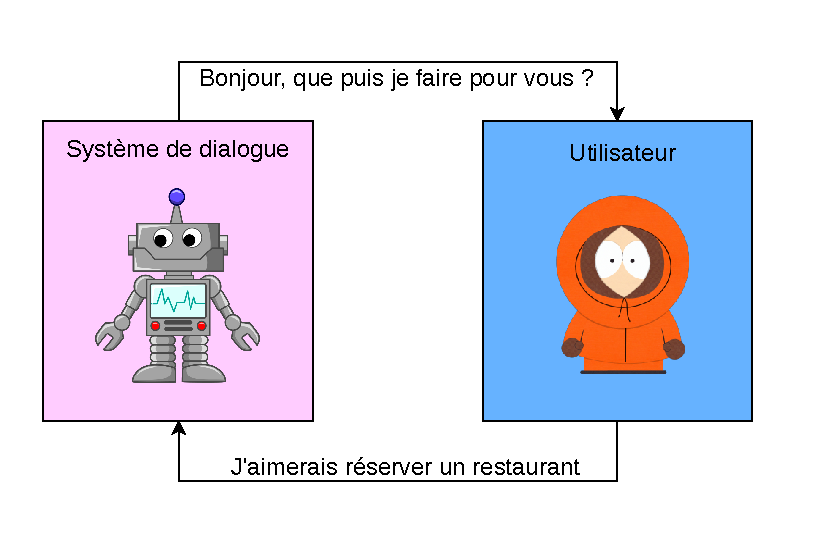
\includegraphics[width=1.0\textwidth]{drawio/out/sds.pdf}
                \end{center}
            \end{column}
        \end{columns}
    \end{frame}

    \begin{frame}{Problématique}
        \begin{columns}
            \begin{column}{0.5\textwidth}
                Besoin de systèmes personalisés.
                \begin{itemize}
                    \item Adaptation aux données de la personne.
                    %  le medecin s'appelle X, la personne habide dans un coin avec certains restaurant
                    \item \textbf{Adaptation au type/habitude de la personne.}
                    % personne agée, enfant, dyslesique, culture (red good chine, red wrong europe) etc
                \end{itemize}
            \end{column}
            \begin{column}{0.5\textwidth}  %%<--- here
                \begin{center}
                    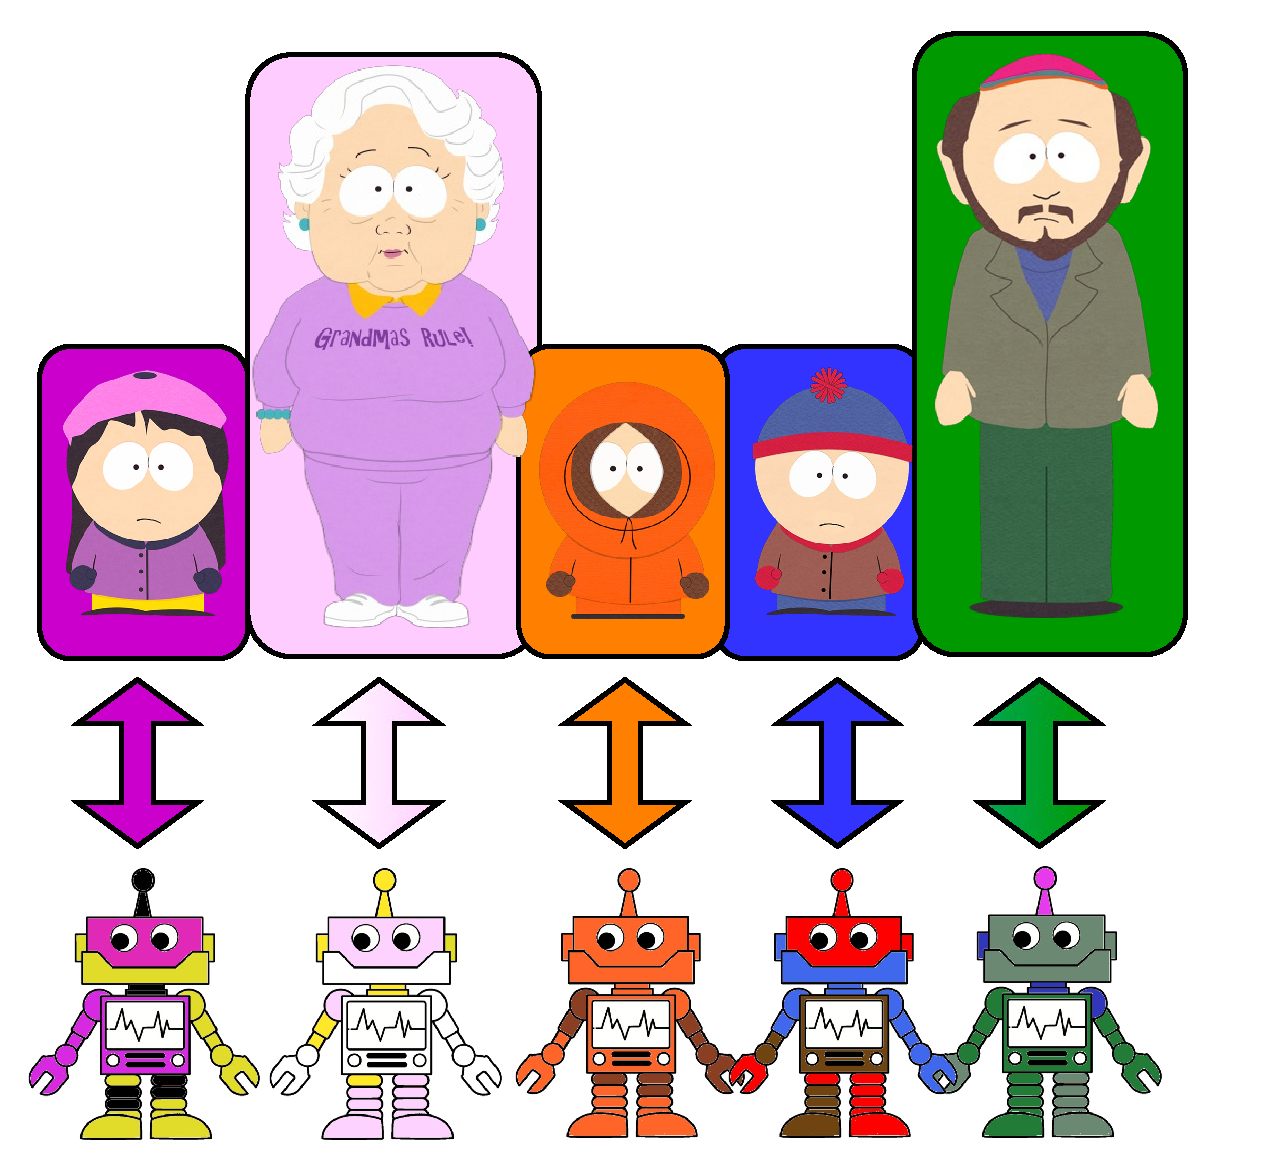
\includegraphics[width=1.0\textwidth]{img/adap1.pdf}
                \end{center}
            \end{column}
        \end{columns}

        %C'est surtout la deuxième problématique qui nous interesse.
        \pause
        \begin{alertblock}{Problématique}
            Comment s'adapter rapidement? Utiliser l'apprentissage par transfert.
            % mais tout d'abord qu'est ce qu'un système de dialogue
        \end{alertblock}

    \end{frame}


    \section{Systèmes de dialogue en détail}



    \subsection{Une architecture modulaire}

    \begin{frame}{Le processus}
        \begin{block}{}
            \invisible{N/A}
        \end{block}
        \begin{figure}
            \centering
            \includegraphics[scale=0.55,page=1]{drawio/out/pipeline-2}
        \end{figure}
    \end{frame}

    \begin{frame}{Le processus}
        \begin{block}{}
            \textit{"Je voudrais réserver un restaurant chinois."}
        \end{block}
        \begin{figure}
            \centering
            \includegraphics[scale=0.55,page=1]{drawio/out/pipeline-1}
        \end{figure}
    \end{frame}

    \begin{frame}{Le processus}
        \begin{block}{}
            Je voulais réserver restaurant chinois $\rightarrow 0.75$
        \end{block}
        \begin{figure}
            \centering
            \includegraphics[scale=0.55,page=1]{drawio/out/pipeline0}
        \end{figure}
    \end{frame}

    \begin{frame}{Le processus}
        \begin{block}{}
            food-type="chinois"
        \end{block}
        \begin{figure}
            \centering
            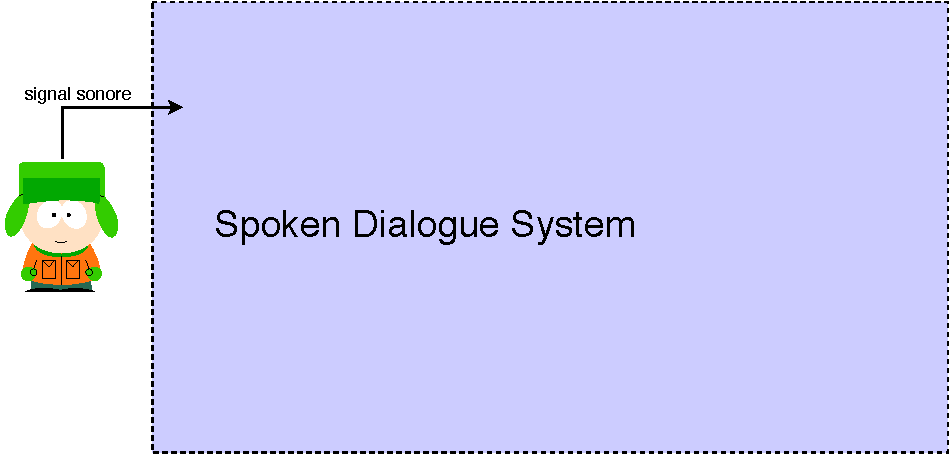
\includegraphics[scale=0.55,page=1]{drawio/out/pipeline1}
        \end{figure}
    \end{frame}

    \begin{frame}{Le processus}
        \begin{block}{}
            food-type="chinois", 0.75, 0.97
        \end{block}
        \begin{figure}
            \centering
            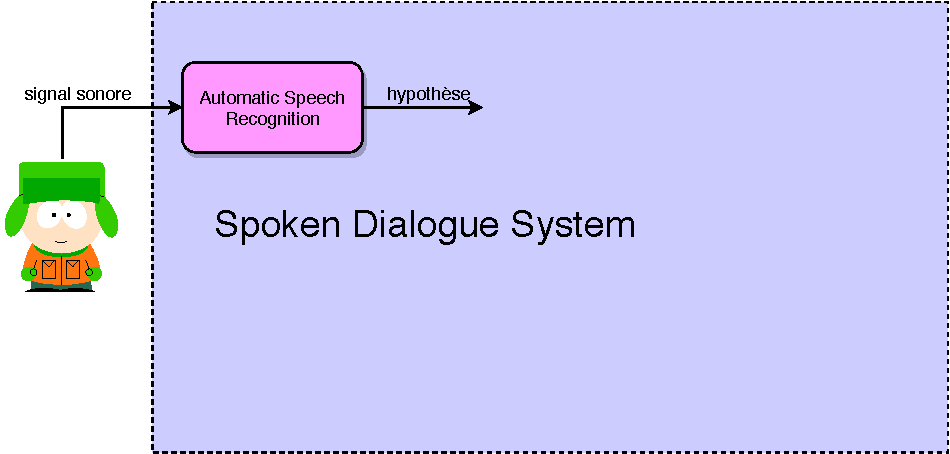
\includegraphics[scale=0.55,page=1]{drawio/out/pipeline2}
        \end{figure}
    \end{frame}



    \begin{frame}{Le processus}
        \begin{block}{  }
            \invisible{N/A}
        \end{block}
        \begin{figure}
            \centering
            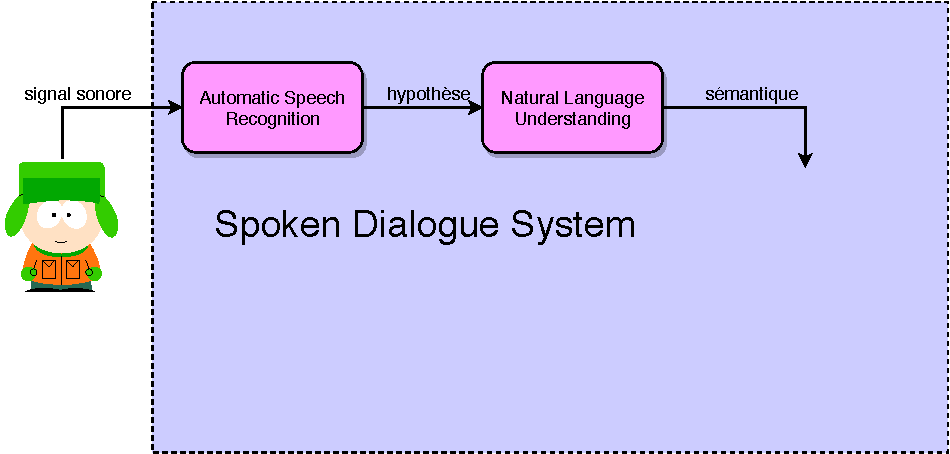
\includegraphics[scale=0.55,page=1]{drawio/out/pipeline3}
        \end{figure}
    \end{frame}


    \begin{frame}{Le processus}
        \begin{block}{  }
            food="chinois", 0.75, 0.97 | venue=None | price=None
        \end{block}
        \begin{figure}
            \centering
            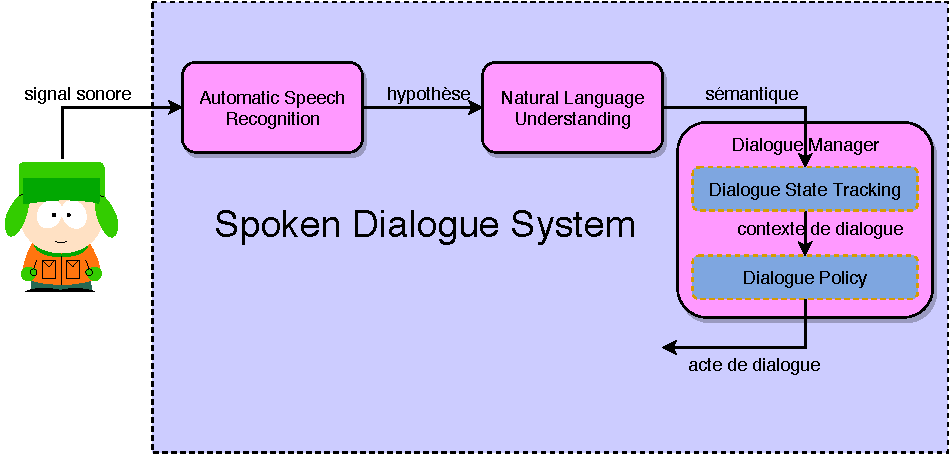
\includegraphics[scale=0.55,page=1]{drawio/out/pipeline4}
        \end{figure}
    \end{frame}


    \begin{frame}{Le processus}
        \begin{block}{}
            expl-conf=(type-food,"chinois")
        \end{block}
        \begin{figure}
            \centering
            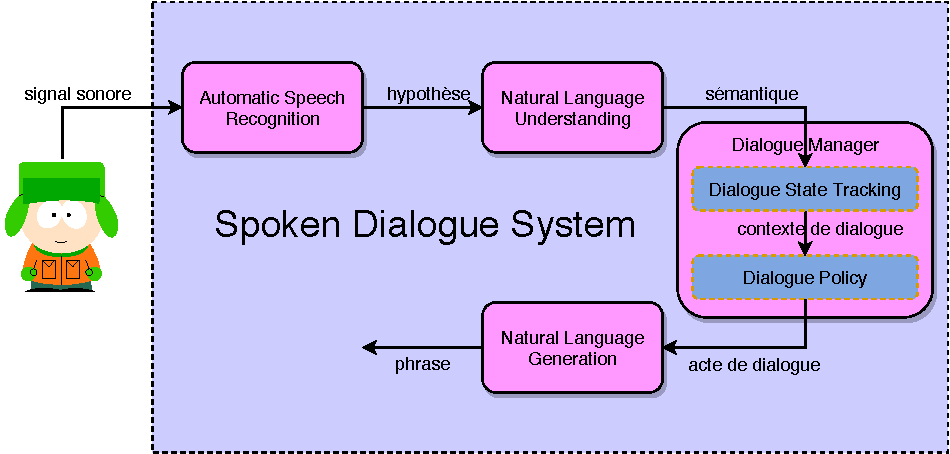
\includegraphics[scale=0.55,page=1]{drawio/out/pipeline5}
        \end{figure}
    \end{frame}

    \begin{frame}{Le processus}
        \begin{block}{}
            Je comprend que vous souhaitez manger chinois, est-ce exact?
        \end{block}
        \begin{figure}
            \centering
            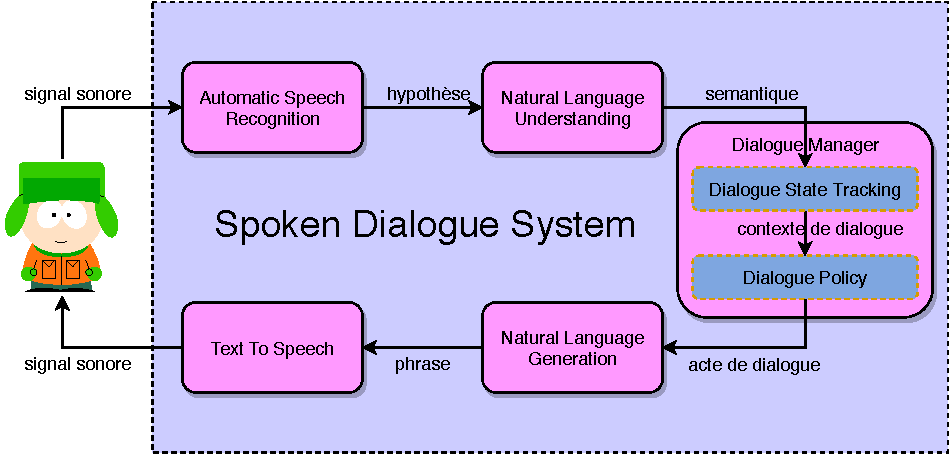
\includegraphics[scale=0.55,page=1]{drawio/out/pipeline6}
        \end{figure}
    \end{frame}

    \begin{frame}{Le processus}
        \begin{block}{}
            \textit{"Je comprend que vous souhaitez manger chinois, est-ce exact?"}
        \end{block}
        \begin{figure}
            \centering
            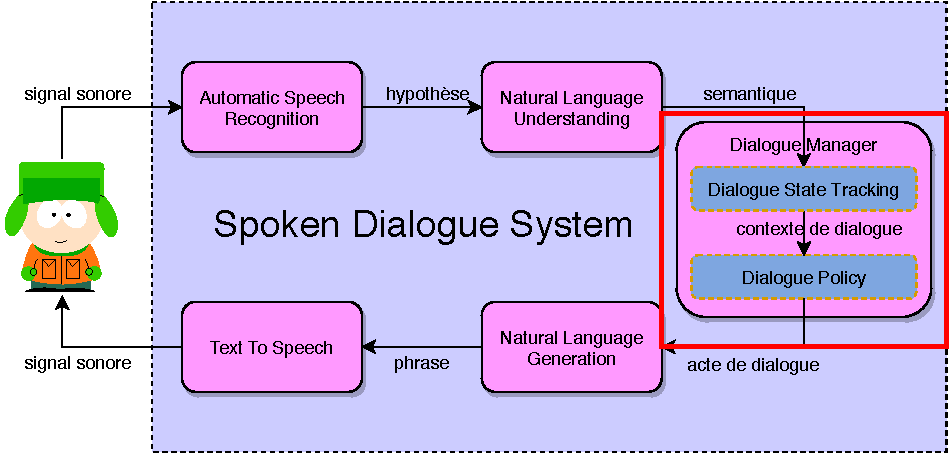
\includegraphics[scale=0.55,page=1]{drawio/out/pipeline7}
        \end{figure}
    \end{frame}

    \begin{frame}{Le processus}
        \begin{block}{}
            \invisible{N/A}
        \end{block}
        \begin{figure}
            \centering
            \includegraphics[scale=0.55,page=1]{drawio/out/pipeline8}
        \end{figure}
    \end{frame}

    \foreach \n in {9,10}{

    \begin{frame}{Prise de Décision Séquentielle}
        \begin{block}{  }
            \invisible{N/A}
        \end{block}
        \begin{figure}
            \centering
            \includegraphics[scale=0.55,page=1]{drawio/out/pipeline\n}
        \end{figure}
    \end{frame}
    }

    \begin{frame}{Prise de Décision Séquentielle}


        \begin{columns}
            \begin{column}{0.5\textwidth}
                \begin{figure}
                    \centering
                    \includegraphics[scale=0.5,page=1]{drawio/out/pipeline12}
                \end{figure}
            \end{column}
            \pause
            \begin{column}{0.5\textwidth}  %%<--- here
                \begin{block}{Succès du dialogue ($r$)}
                    Si contraintes de l'utilisateur sont remplies, sans erreurs.
                \end{block}

                \begin{block}{Actes de dialogues ($a$)}
                    Request, repeat, explicit/implicit-confirm ...
                \end{block}

                \begin{block}{Etats ($s$)}
                    \begin{itemize}
                        \item Actions du système.
                        \item Scores de confiance.
                        \item Actions de l'utilisateur.
                    \end{itemize}
                \end{block}
            \end{column}
        \end{columns}
        \pause
        \begin{alertblock}{}
            Comment décider l'action en fonction de l'état courant ?
        \end{alertblock}

    \end{frame}



    \subsection{Apprentissage par renforcement}
    \begin{frame}{Processus de Decision Markovien}

        Un MDP est un tuple $\langle{}\cS,\cA,\reward,\transition,\discountfactor\rangle{}$ où:
        \begin{itemize}
            \item  $\cS$ est l'espace des états,
            \item  $\cA$ est l'espace des actions,
            \item $\reward: \cS\times\cA \rightarrow \Real$ est la fonction de récompense,
            \item $\transition: \cS\times\cA \rightarrow \cM(\cS)$ est la fonction de transition,
            \item $\discountfactor$ est le facteur d'actualisation.
        \end{itemize}

    \end{frame}

    \begin{frame}{Résoudre un MDP}

        \begin{block}{Définitions}
            \begin{itemize}
                \item  $\policy\in\cM(\cA)^{\cS}$ % that maps states to actions
                \item  $\return^{\policy} = \sum_{\indextransition=0}^\infty \discountfactor^{\indextransition} \reward(s_{\indextransition},a_{\indextransition})$
                % expliquer s_i et a_i

            \end{itemize}
        \end{block}
        \pause
        \begin{block}{Optimalité}
            \begin{itemize}
                \pause\item $\policy^* = \argmax\limits_{\policy} \mathbb{E}_{\policy} [\return^{\policy}|s_0=s,a_0=a]\ \forall (s,a) \in \cS\times\cA$
                \pause\item $\Q^*(s,a)=\reward(s,a) +\discountfactor \sum_{s'\in \cS}[\transition(s,a,s')\max_{a'\in \cA}\Q^*(s',a')] = \bo Q^*.$
                % It exists a unique function, denoted as $\Q^*$, that verifies the Bellman Optimality equation:

                \pause\item $\optimalpolicy(s) \in \argmax\limits_{a\in \cA} \Q^*(s,a)$ est optimale.
            \end{itemize}
        \end{block}

    \end{frame}

    \begin{frame}{Algoritmes}

        \begin{block}{Value-Iteration}
            \begin{itemize}
                \item $Q \leftarrow \mathbf{0}$
                \item $Q(s,a) \leftarrow \bo Q(s,a)\ \forall (s,a)$ jusqu'à convergence
                \item Renvoyer $\pi(s) = \argmax\limits_{a} Q(s,a)$
            \end{itemize}
        \end{block}
        \pause
        \begin{alertblock}{}
            \begin{itemize}
                \item Comment calculer $\bo Q$ si $\transition$ et $\reward$ sont inconnues?
                \begin{itemize}
                    \item Estimateur avec $\mathcal{D}=\{(s_i,a_i,r_i,s_i')\}_{i\in[0,N]}$
                \end{itemize}
                \item Comment calculer $Q\ \forall (s,a) \in \cS\times\cA$ si $S$ est très grand voir continu ?
                \begin{itemize}
                    \item Approximation de fonction
                \end{itemize}
            \end{itemize}

        \end{alertblock}
        \pause
        \begin{block}{Fitted-Q}
            \begin{itemize}
                \item $Q \leftarrow \mathbf{0}$
                \item $Q \leftarrow \Gamma(\{s_{\indextransition},a_{\indextransition}\}_{{\indextransition}\in \T},\{r_{\indextransition} + \discountfactor  \max_{a'\in\cA} \Q(s'_i,a')\}_{{\indextransition} \in \T})$ jusqu'à convergence
                \item Retourner $\pi(s) = \argmax\limits_{a} Q(s,a)$
            \end{itemize}
        \end{block}


    \end{frame}

    \begin{frame}{}


        \begin{alertblock}{}
            Comment apprendre face à un utilisateur inconnu?
        \end{alertblock}


        \begin{itemize}
            \item \cmoins Amasser des transitions et apprendre en ligne (\textit{from scratch})
            \item \cplus Mise à profit de notre expérience avec d'autres utilisateurs
            \begin{itemize}
                \item Apprentissage par transfert
            \end{itemize}

        \end{itemize}


    \end{frame}

    \subsection{Apprentissage par Transfert}
    \begin{frame}{Pourquoi transférer ?}

        \begin{figure}
            \begin{center}
                \subfloat[Performance au démarrage]{
                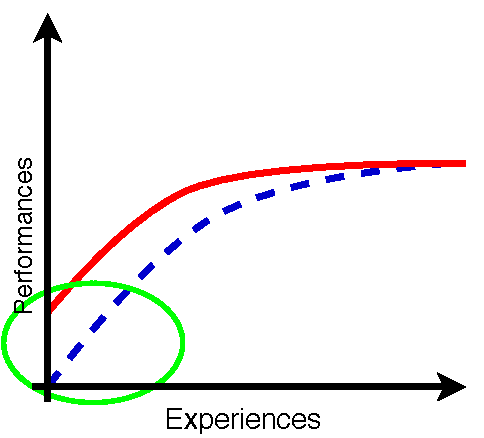
\includegraphics[width=0.33\textwidth]{../sources/dm-tl/objectives-jumpstart}
                \label{fig:objectives-jumpstart}
                }
                \subfloat[Performance d'apprentissage]{
                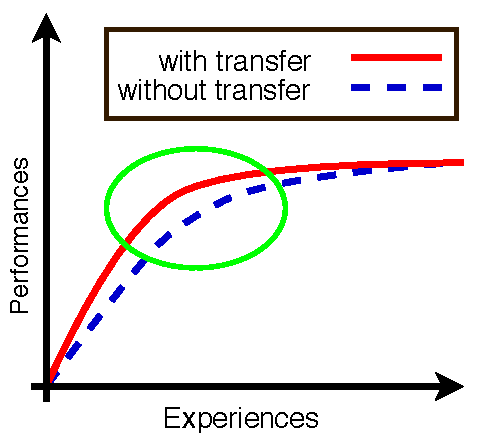
\includegraphics[width=0.33\textwidth]{../sources/dm-tl/objectives-learn}
                \label{fig:objectives-learn}
                }
                \subfloat[Performance asymptotique]{
                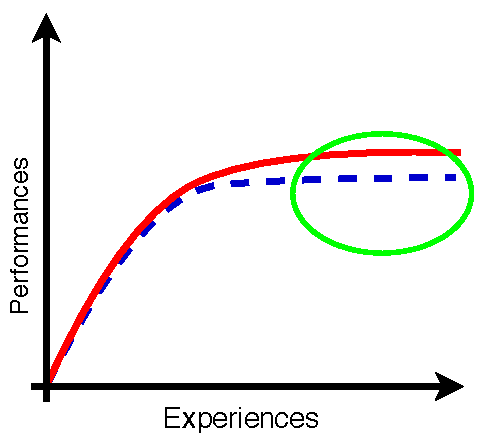
\includegraphics[width=0.33\textwidth]{../sources/dm-tl/objectives-asymptote}
                \label{fig:objectives-asymptote}
                }
                \caption{Les objectifs de l'apprentissage par transfert~\parencite{langley2006}}
                \label{fig:objectives}
            \end{center}
        \end{figure}

    \end{frame}

    \begin{frame}{Les différentes formes de transfert}
        \begin{itemize}
            \item Utiliser une ou des tâches sources,
            \item pour apprendre une ou des tâches cibles.
        \end{itemize}


        \begin{table}
            \centering
            \resizebox{0.7\textwidth}{!}{
            \begin{tabular}{lll}
                \hline
                & Connaissance & Cadre \\ \hline
                \textbf{cross domain} &&\\
                \hline
                \cite{Gasic2013}&transitions/politique & \makecell[l]{mono} \\
                \cite{Keizer2018-tl-dialogue}& politique& \makecell[l]{generique} \\
                \cite{Chen2018-tl-dialogue}& politique & \makecell[l]{generique}\\
                \cite{Ilievski2018-tl-dialogue}& politique & \makecell[l]{mono}\\
                \hline
                \textbf{user adaptation} &&\\
                \hline
                \cite{casanueva2015-tl-dialogue}& transitions/politique & \makecell[l]{multi}\\
                \cite{Genevay2016}&\makecell[l]{transitions, politique} &\makecell[l]{multi}\\
                \cite{Mo2018-tl-dialogue-PETAL}&$\Q$-fonction, DST &\makecell[l]{generique}\\
                \hline
            \end{tabular}
            }
        \end{table}


    \end{frame}

    \begin{frame}{Contributions}
        %On va explorer
        Deux directions, toutes deux exploitant l'apprentissage par transfert.
        \pause
        \begin{itemize}
            \item Approche classique, avec l'utilisation d'outils existants et leur mise à l'echelle.
            \begin{itemize}
                \item Processus complet pour l'adaptation ~\parencite{ncarrara-online}
                \item Transfer Deep-$Q$-Network
            \end{itemize}
            \pause
            \item Approche plus conservatrice, en mettant en avant la notion de risque dans la conversation.
            \begin{itemize}
                \item Budgeted Reinforcement Learning~\parencite{ncarrara-brl}
                \item $\epsilon$-safe~\parencite{ncarrara-safe}
            \end{itemize}
        \end{itemize}


    \end{frame}

    \section{Passage à l'échelle de l'apprentissage par transfert}

    \subsection{Un processus complet pour l'adaptation à l'utilisateur}



    \foreach \n in {0,1,2,3,4,5,6,7,8,9,10,11,13,14}{
    \begin{frame}{Le processus}
        %{but what if the system database grow ? bandit useless}
        \begin{figure}
            \begin{center}
                \includegraphics[width=0.75\textwidth]{img/dataflowRobot\n.pdf}
            \end{center}
        \end{figure}
    \end{frame}
    }

    \begin{frame}{\textsc{PD-distance}}
        \begin{figure}
            \begin{center}
                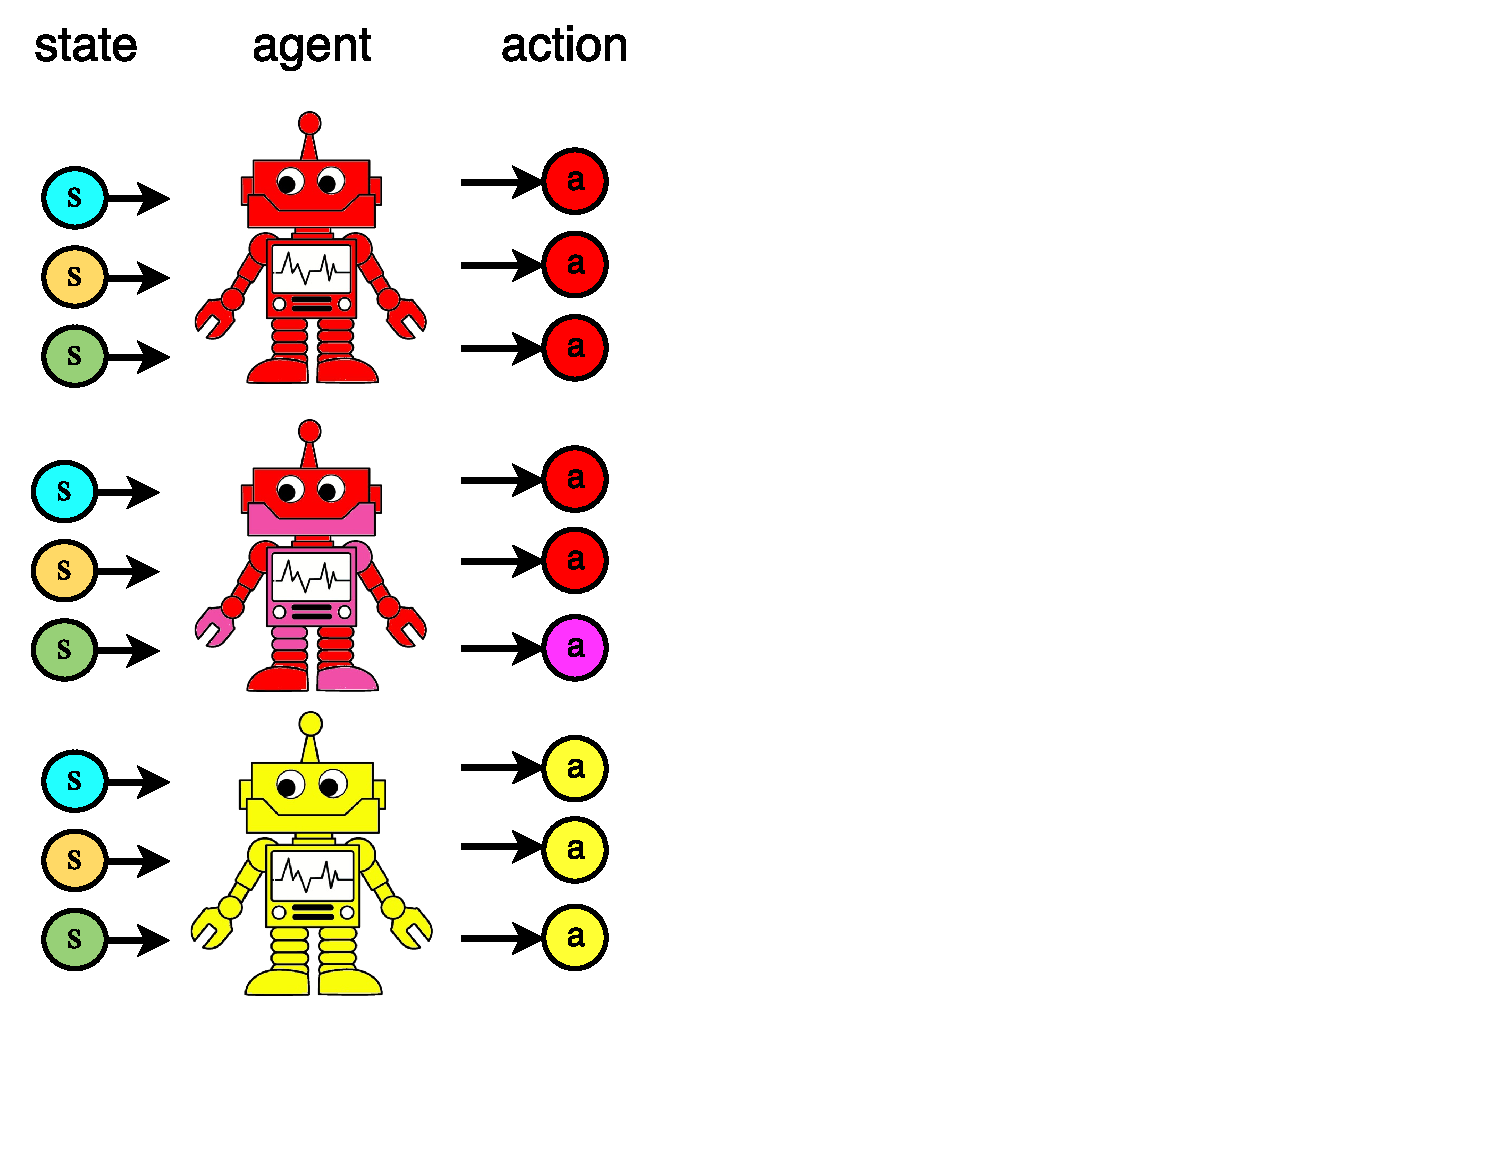
\includegraphics[width=1.0\textwidth]{img/pddistance0.pdf}
            \end{center}
        \end{figure}
    \end{frame}

    \begin{frame}{\textsc{PD-distance}}
        \begin{figure}
            \begin{center}
                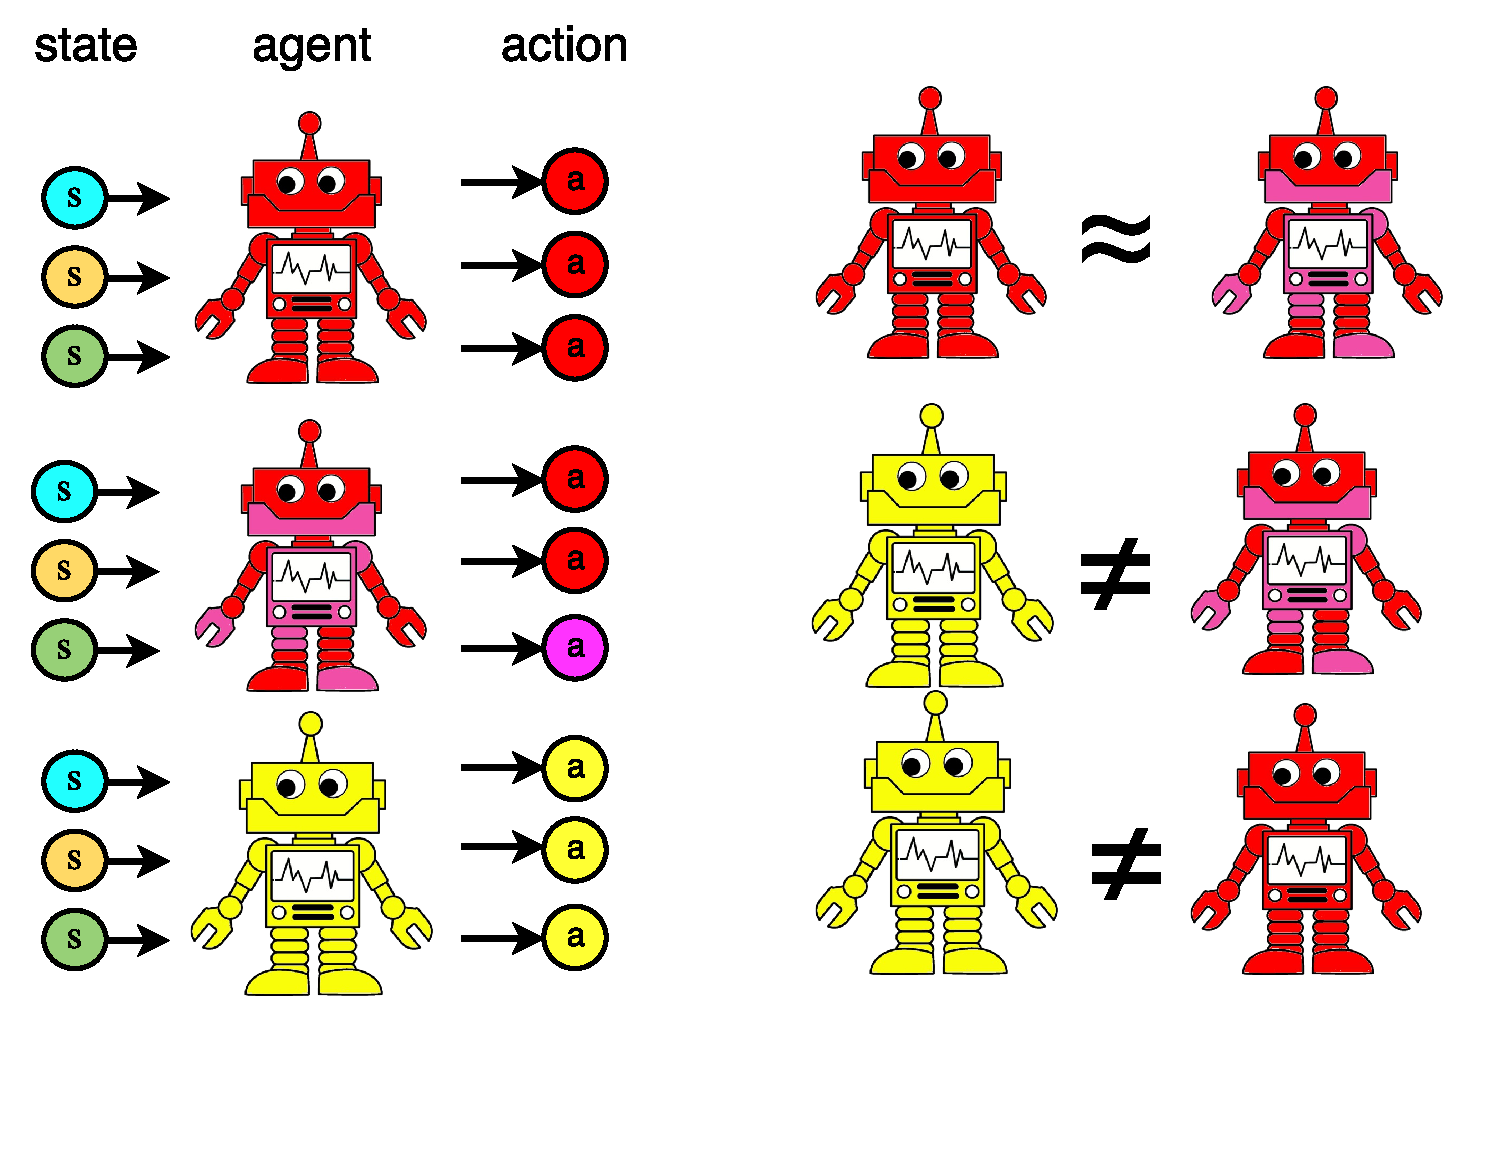
\includegraphics[width=1.0\textwidth]{img/pddistance.pdf}
            \end{center}
        \end{figure}
    \end{frame}
    \foreach \n in {0,1,2,3,4}{
    \begin{frame}{\textsc{PD-distance} et norme euclidienne}
        \begin{figure}
            \begin{center}
                \includegraphics[width=1.0\textwidth]{img/euclide\n.pdf}
            \end{center}
        \end{figure}
    \end{frame}
    }

    \begin{frame}{\textsc{K-means}}
        \begin{figure}
            \begin{center}
                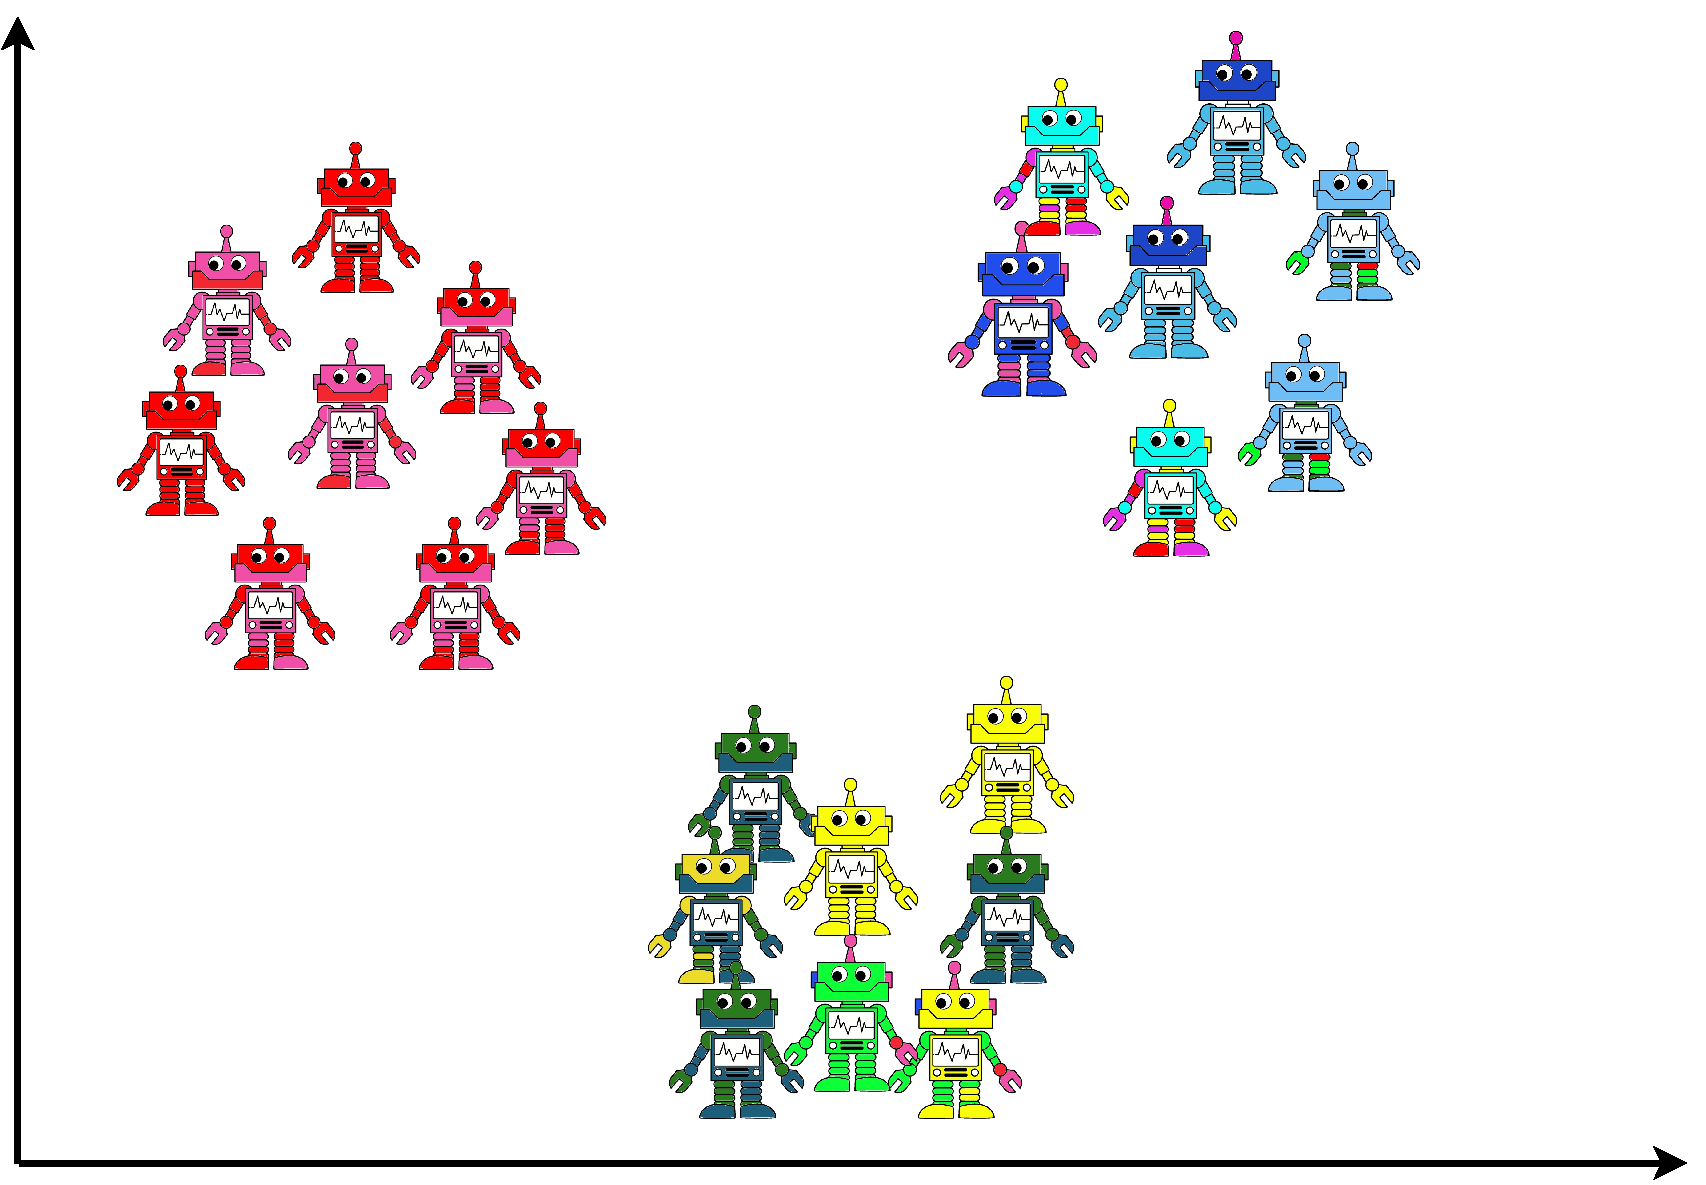
\includegraphics[width=0.85\textwidth]{img/clustering.pdf}
            \end{center}
        \end{figure}
    \end{frame}

    \foreach \n in {0}{
    \begin{frame}{\textsc{K-means}}
        \begin{figure}
            \begin{center}
                \includegraphics[width=0.85\textwidth]{img/kmeans\n.pdf}
            \end{center}
        \end{figure}
    \end{frame}
    }
    \begin{frame}{\textsc{K-medoids}}
        \begin{figure}
            \begin{center}
                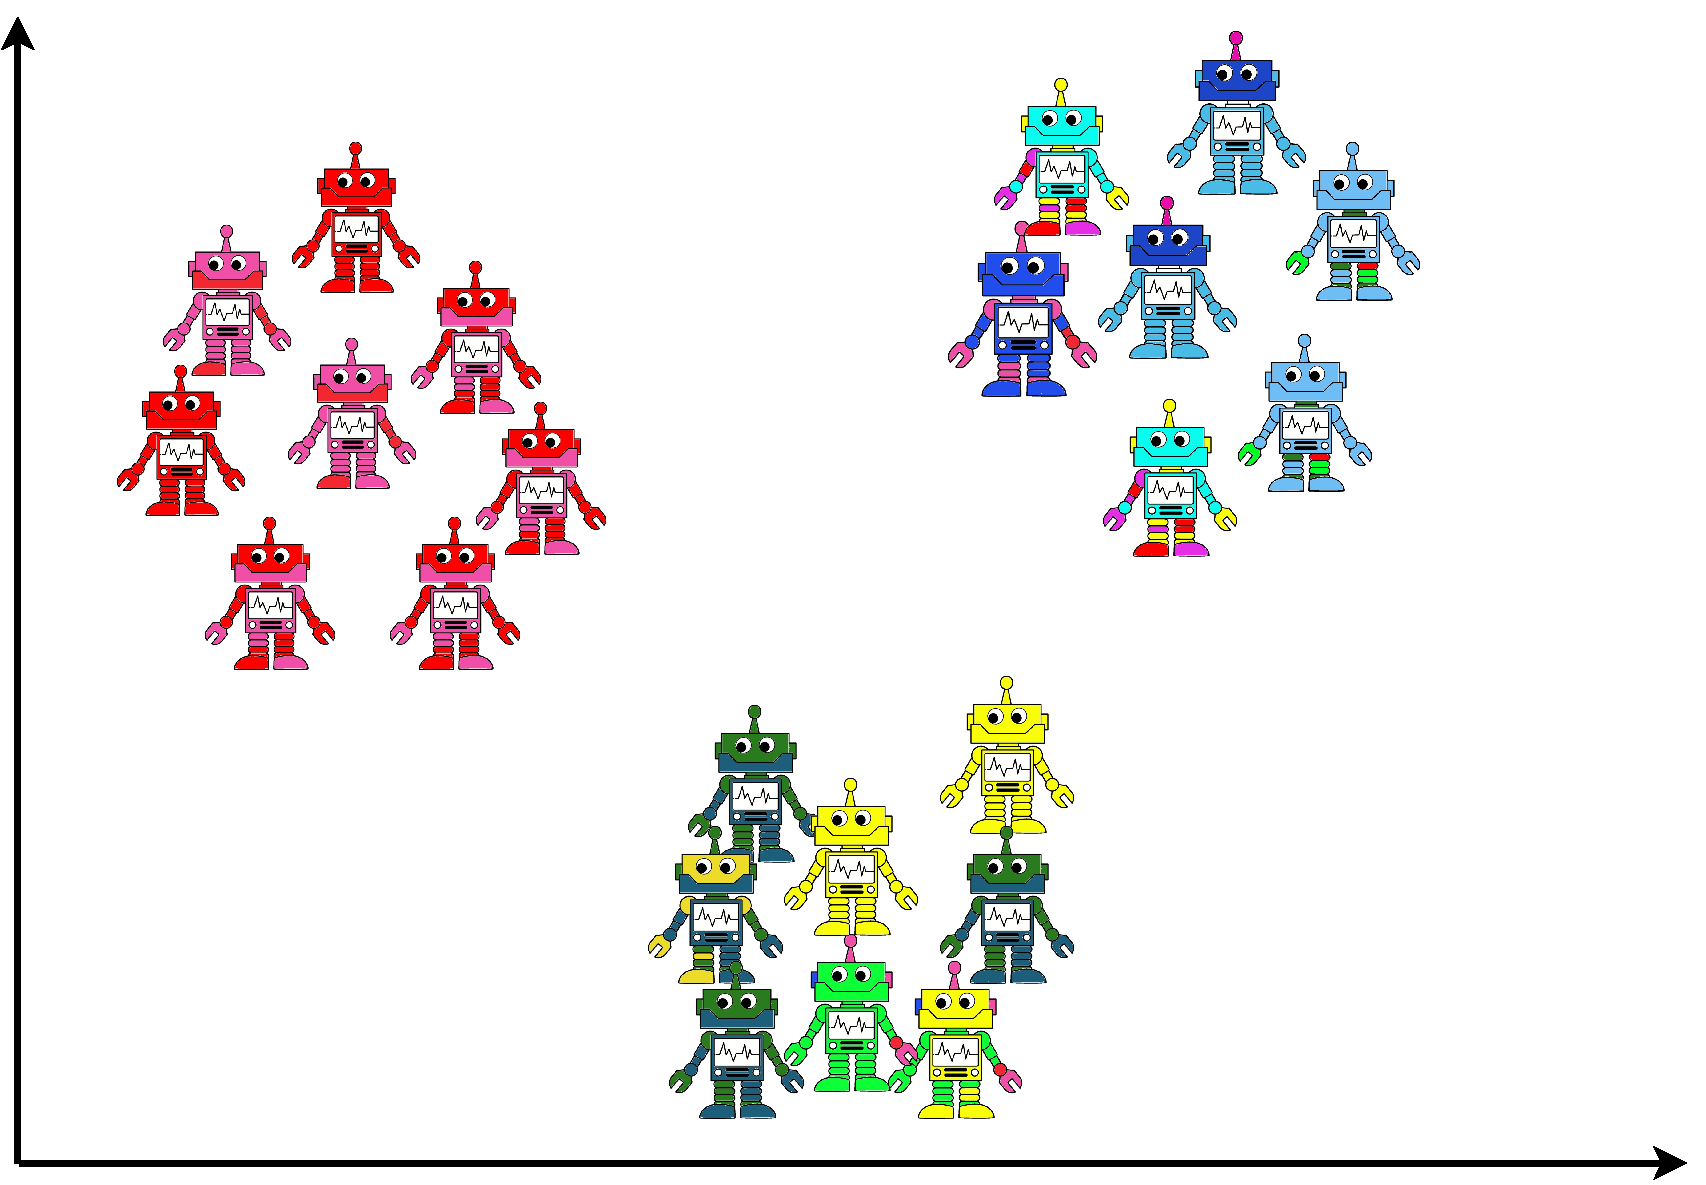
\includegraphics[width=0.85\textwidth]{img/clustering.pdf}
            \end{center}
        \end{figure}
    \end{frame}

    \begin{frame}{\textsc{K-medoids}}
        \begin{figure}
            \begin{center}
                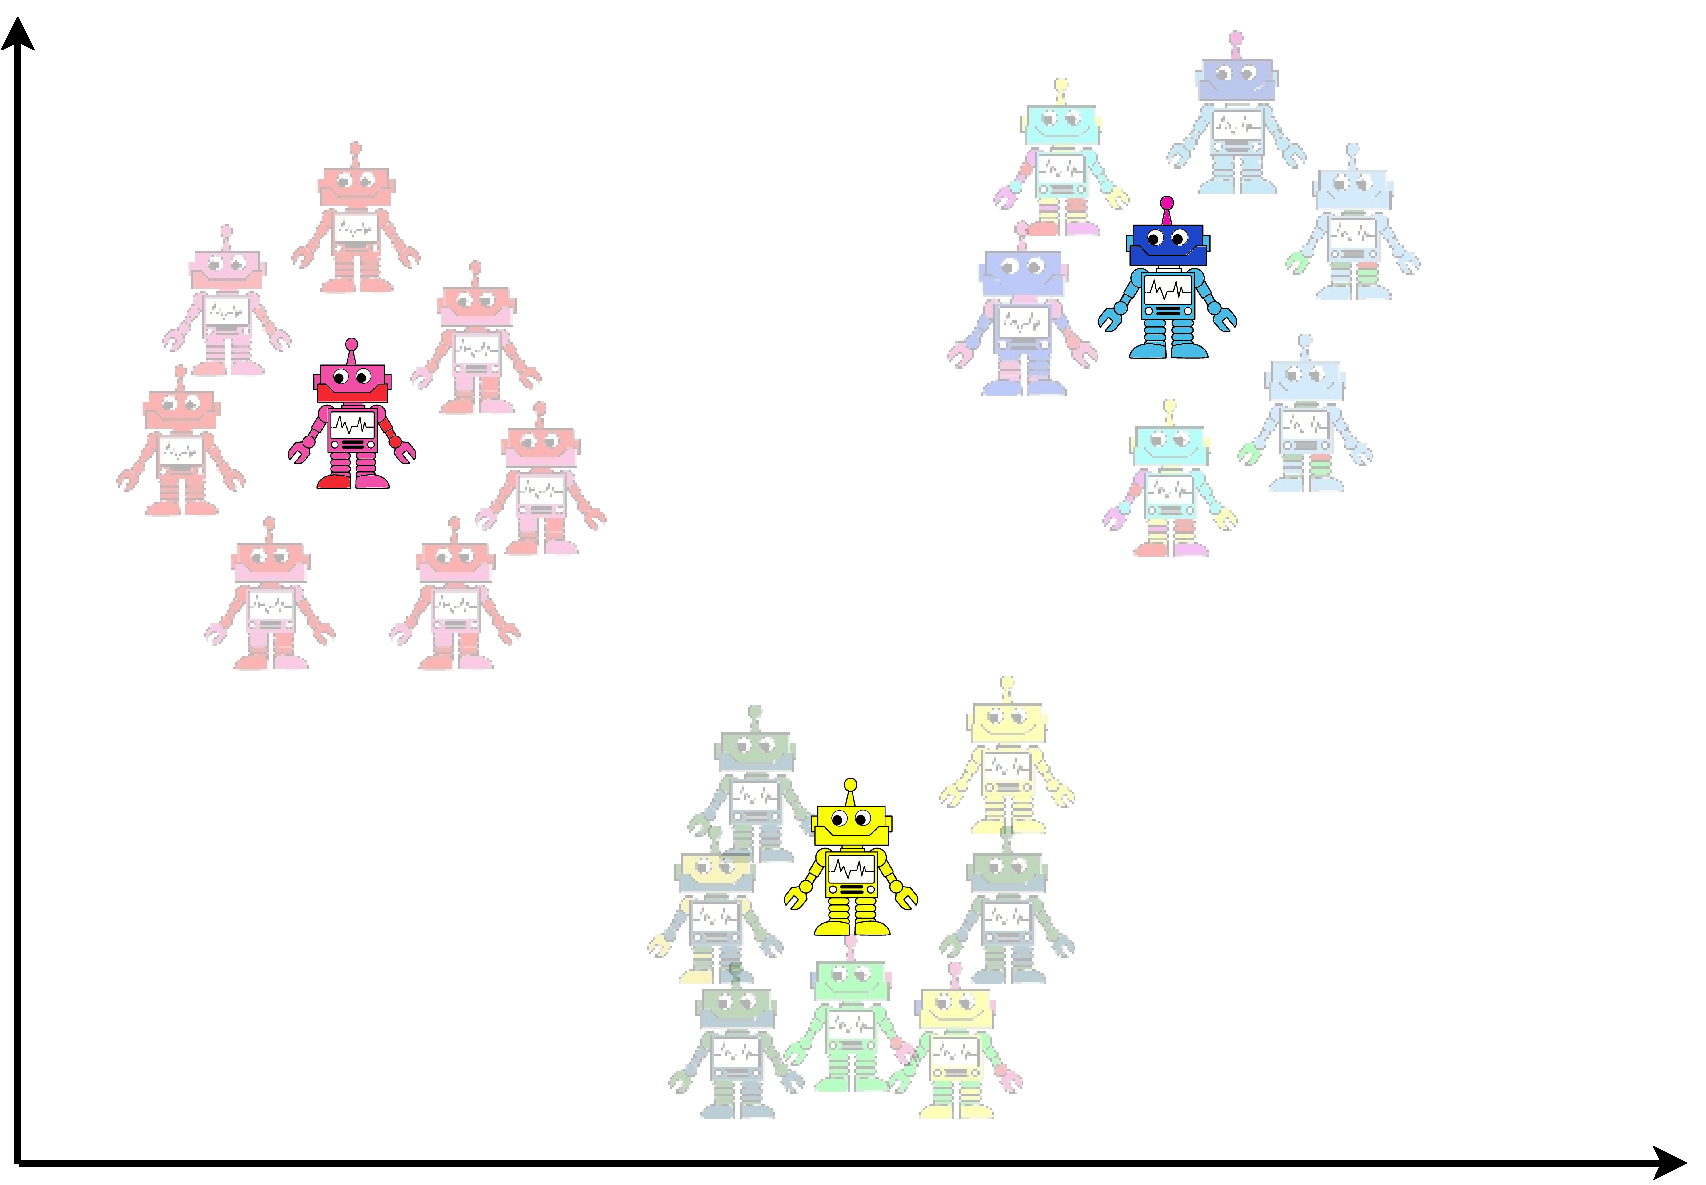
\includegraphics[width=0.85\textwidth]{img/kmedoids.pdf}
            \end{center}
        \end{figure}
    \end{frame}

    \begin{frame}{Expériences}
        \begin{block}{Environnement}
            The negotiation dialogue game~\parencite{Laroche2016}.
        \end{block}

        \begin{figure}
            \begin{center}
                \setlength{\tabcolsep}{0.15em}
                \begin{tabular}{|l|c|c|c|c||c|c|c|c|c|c|c|c|c|}
                    \hline
                    \backslashbox{u}{s}& type & $c_{\top}$ & $c_{\bot}$ & x&vspu1 & vspu2 & vspu3 & vspu4 & vspu5 & vspu6 & vspu7   \\
                    \hline

                    pu1 & DU & 1 & -1 & 0.1 &  \textbf{0,62 }& 0,44 & 0,46 & 0,40 & 0,40 &0,40 & 0,59    \\
                    pu2 & DU & 5 & -5 & 0.1 & 0,53 &  \textbf{0,82}  & 0,81& 0,51 & 0,70 & 0,41 & 0,71 \\
                    pu3 & DU & 5 & -5 & 0.2& 0,53 &  \textbf{0,81} & \textbf{0,81}  & 0,52 & 0,72 & 0,42 & 0,71  \\
                    pu4 & RU & 5 & -5 & 0.1& 0,42 & 0,94 & 0,94 & \textbf{1,00}& 0,92 & 0,85 & 0,94 \\
                    pu5 & ARPBU & 1 & -1& &0,84& 0,98 & 1,00 & 1,11 &\textbf{1,16}& 1,13 & 1,05    \\
                    pu6 & AAU & 1 & -1 & &0,95 & 1,06 & 1,07 & 1,29 & 1,27 &\textbf{1,30} & 1,06 \\
                    pu7 & SAOTU & 1 & -1& &0,43 & 0,26& 0,27 & 0,10 & 0,18 & 0,03 &\textbf{ 0,58}  \\
                    \hline
                \end{tabular}
            \end{center}
            \caption{Comparaison croisée}
        \end{figure}
    \end{frame}

    \begin{frame}{Expériences}


        \begin{figure}
            \captionsetup[subfigure]{labelformat=empty}
            \begin{center}
                \subfloat[Score]{
                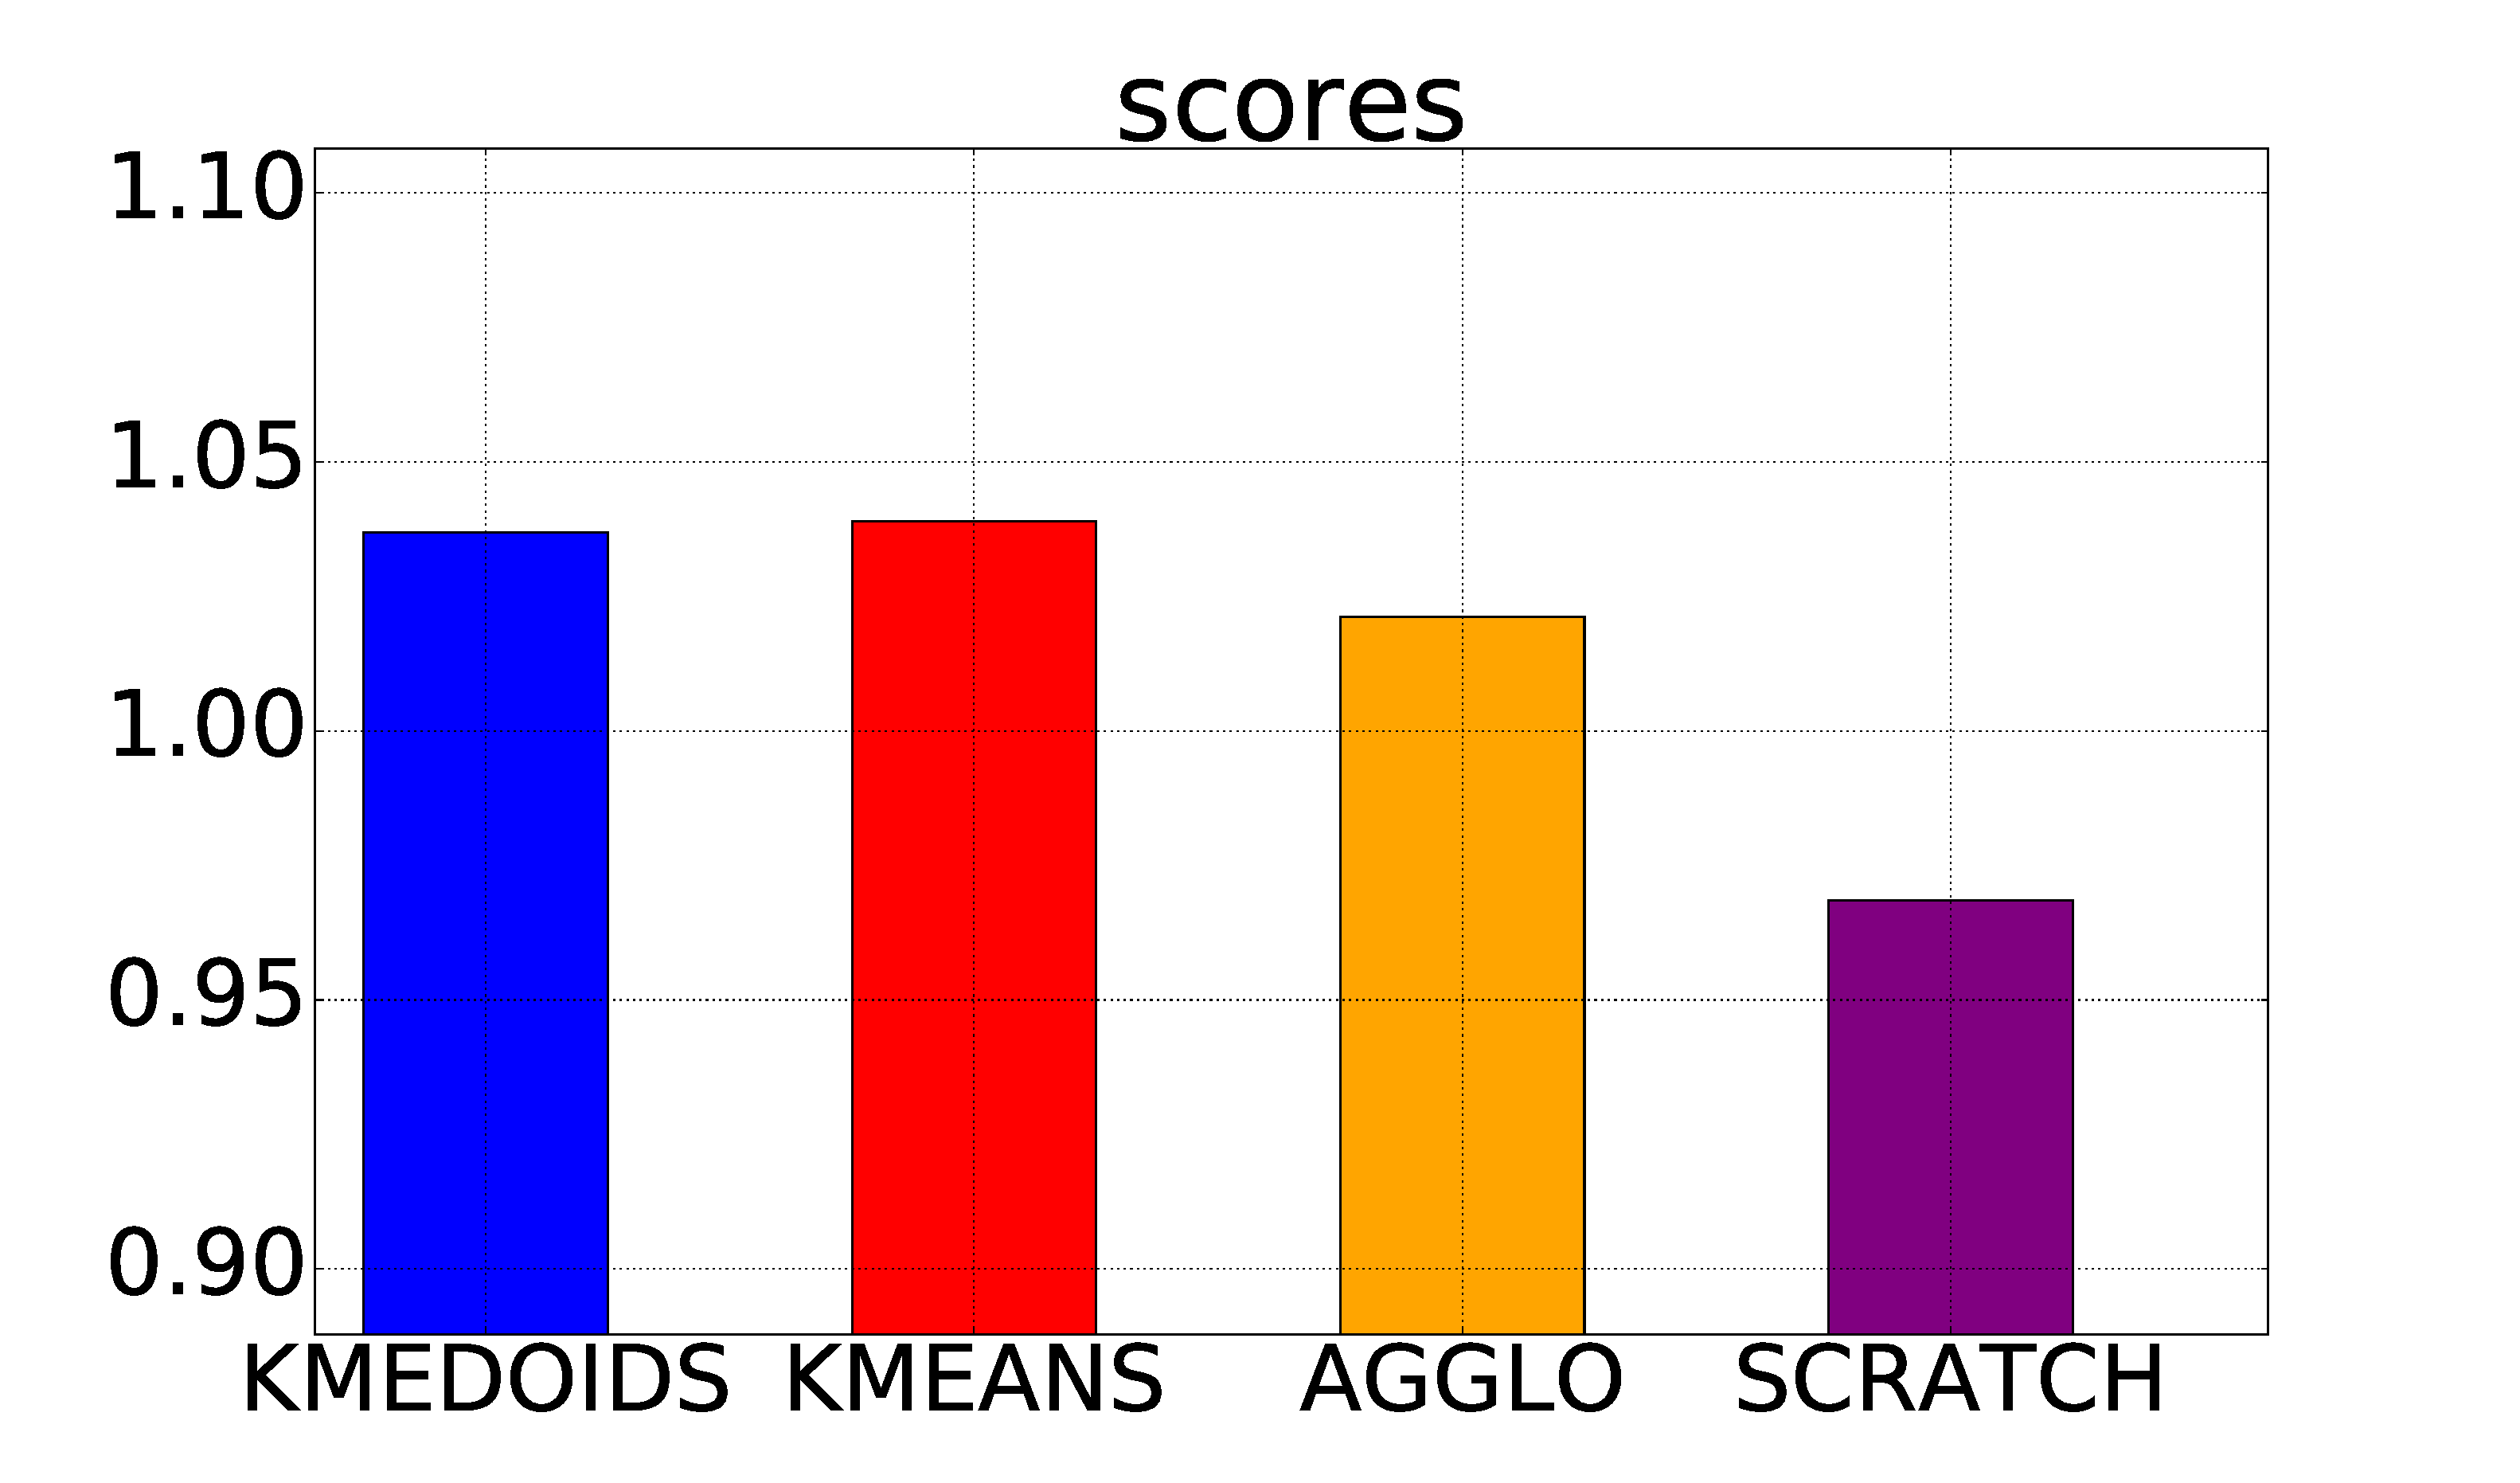
\includegraphics[width=0.33\textwidth]{img/handcraftedScores.pdf}
                }
                \subfloat[Longueur du dialogue]{
                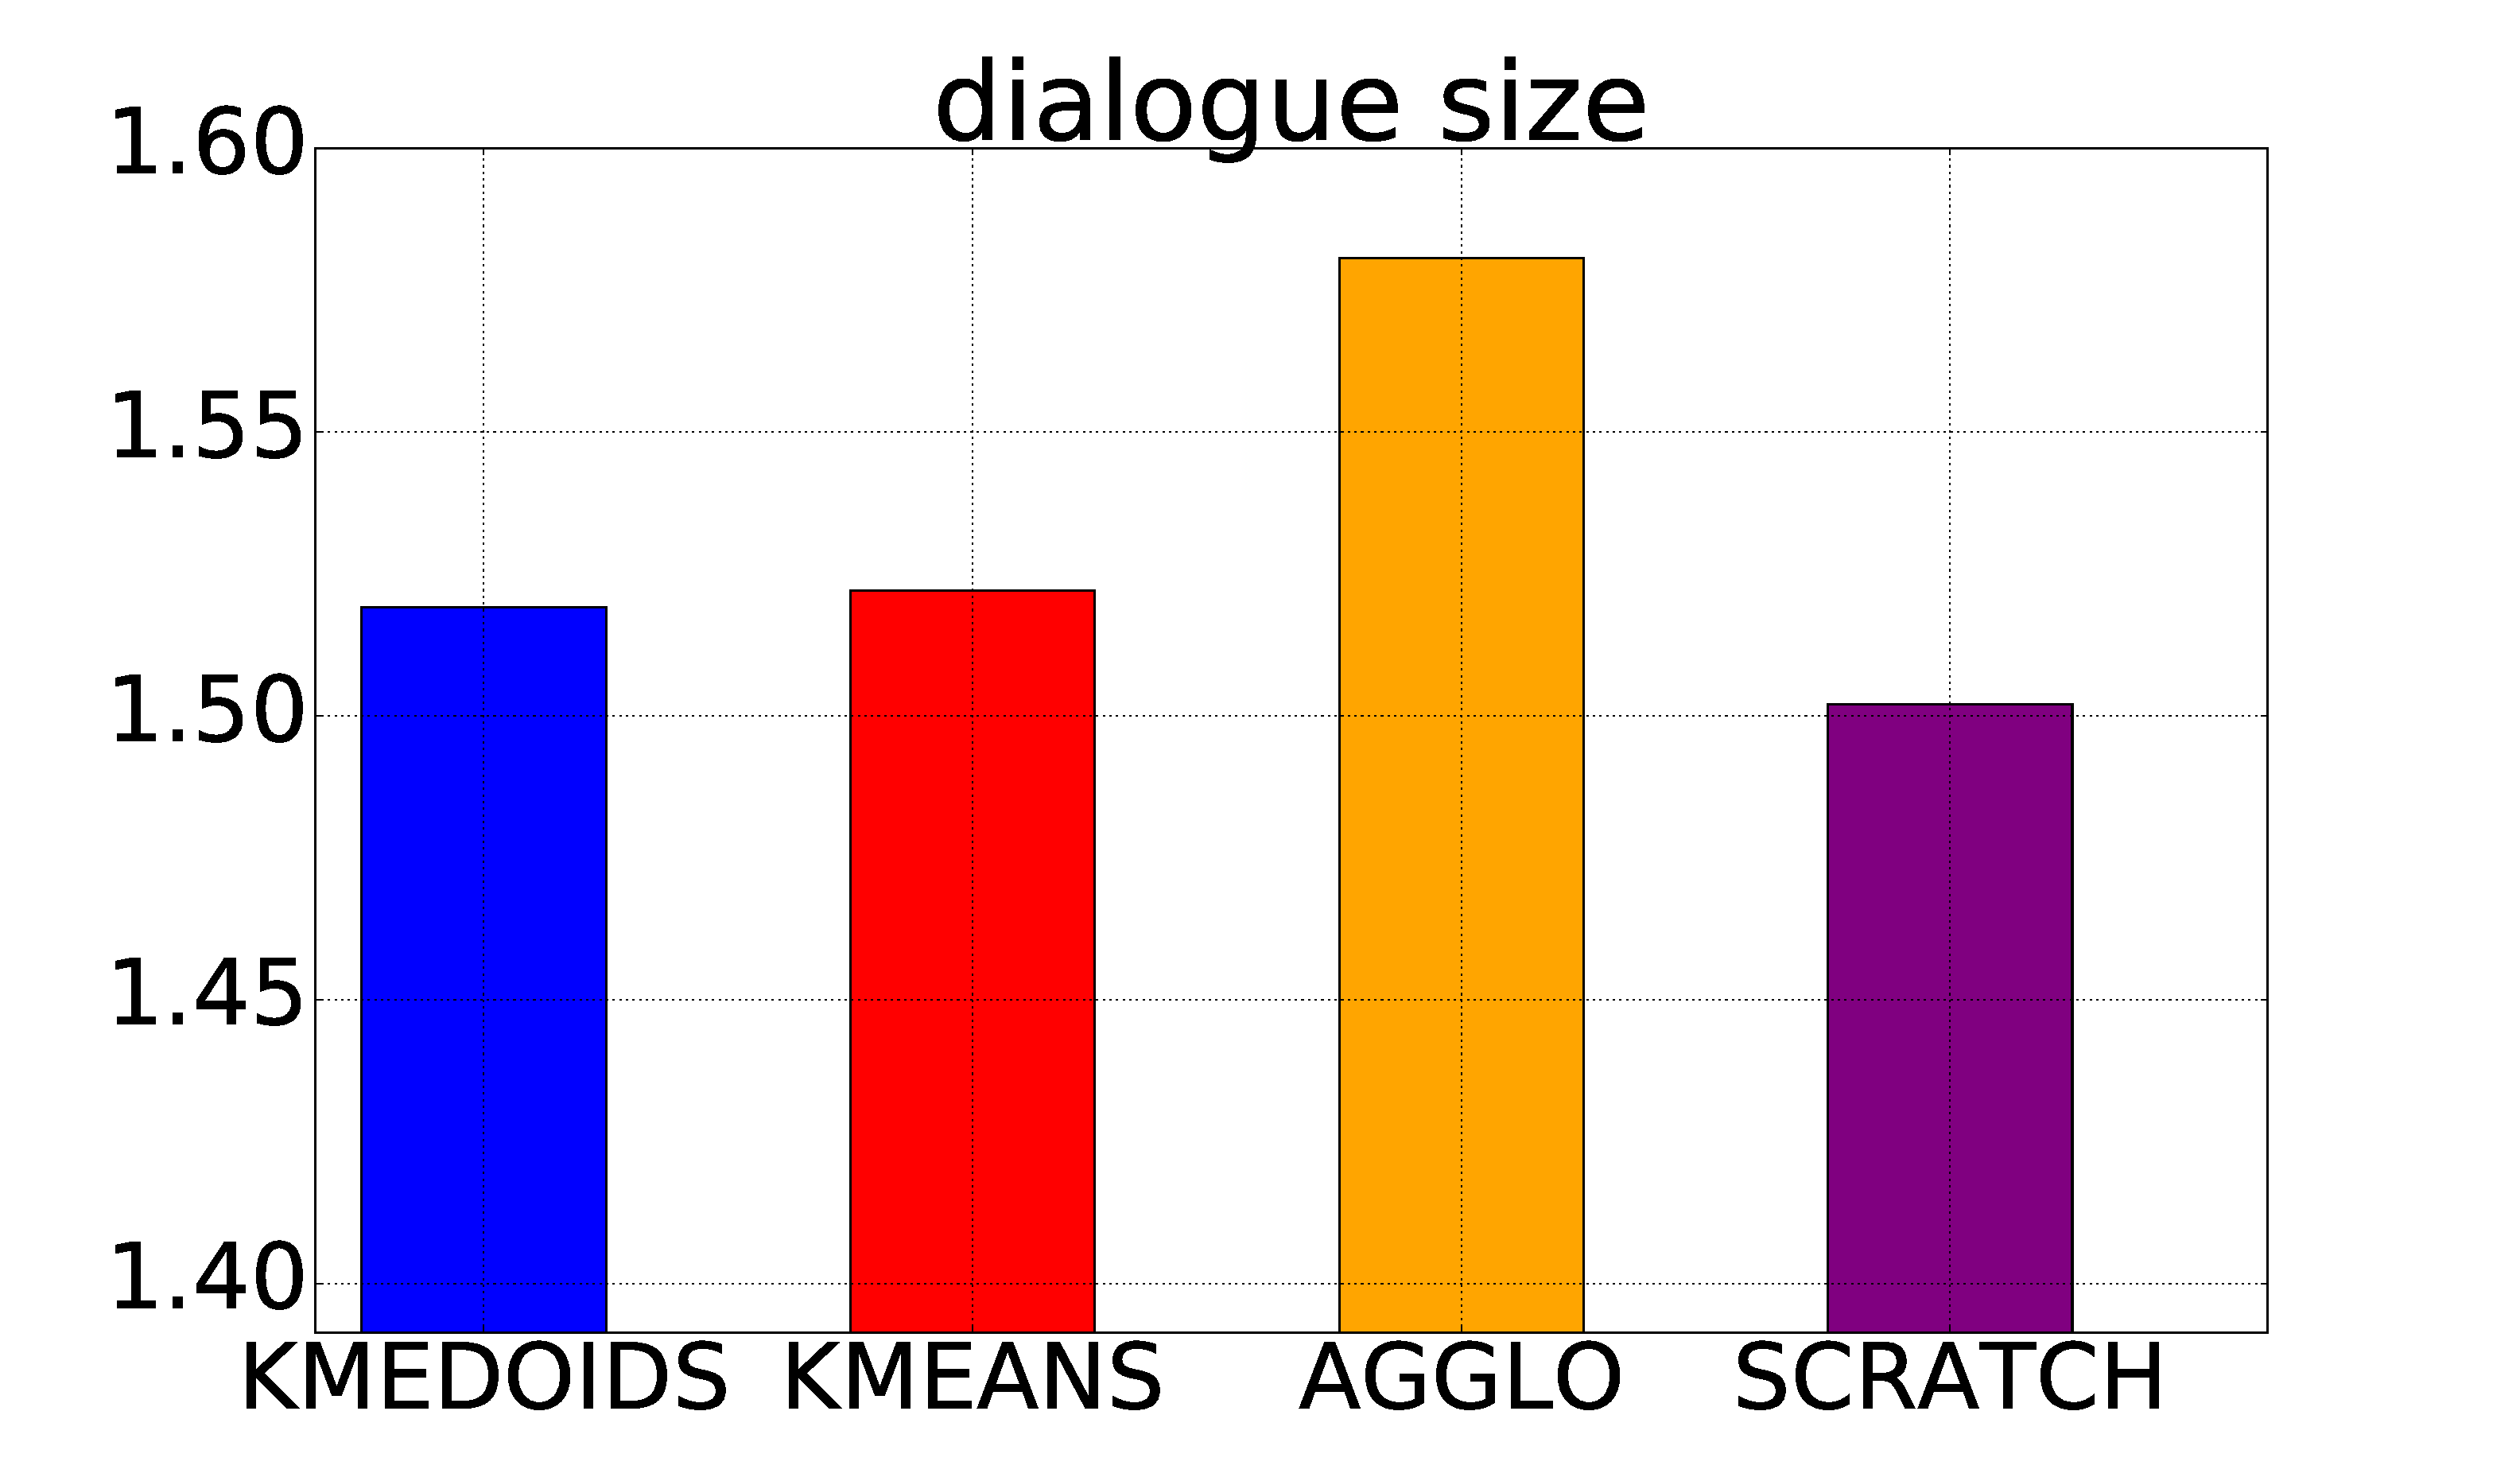
\includegraphics[width=0.33\textwidth]{img/handcraftedDialoguesize.pdf}
                }
                \subfloat[Réussite de la tâche]{
                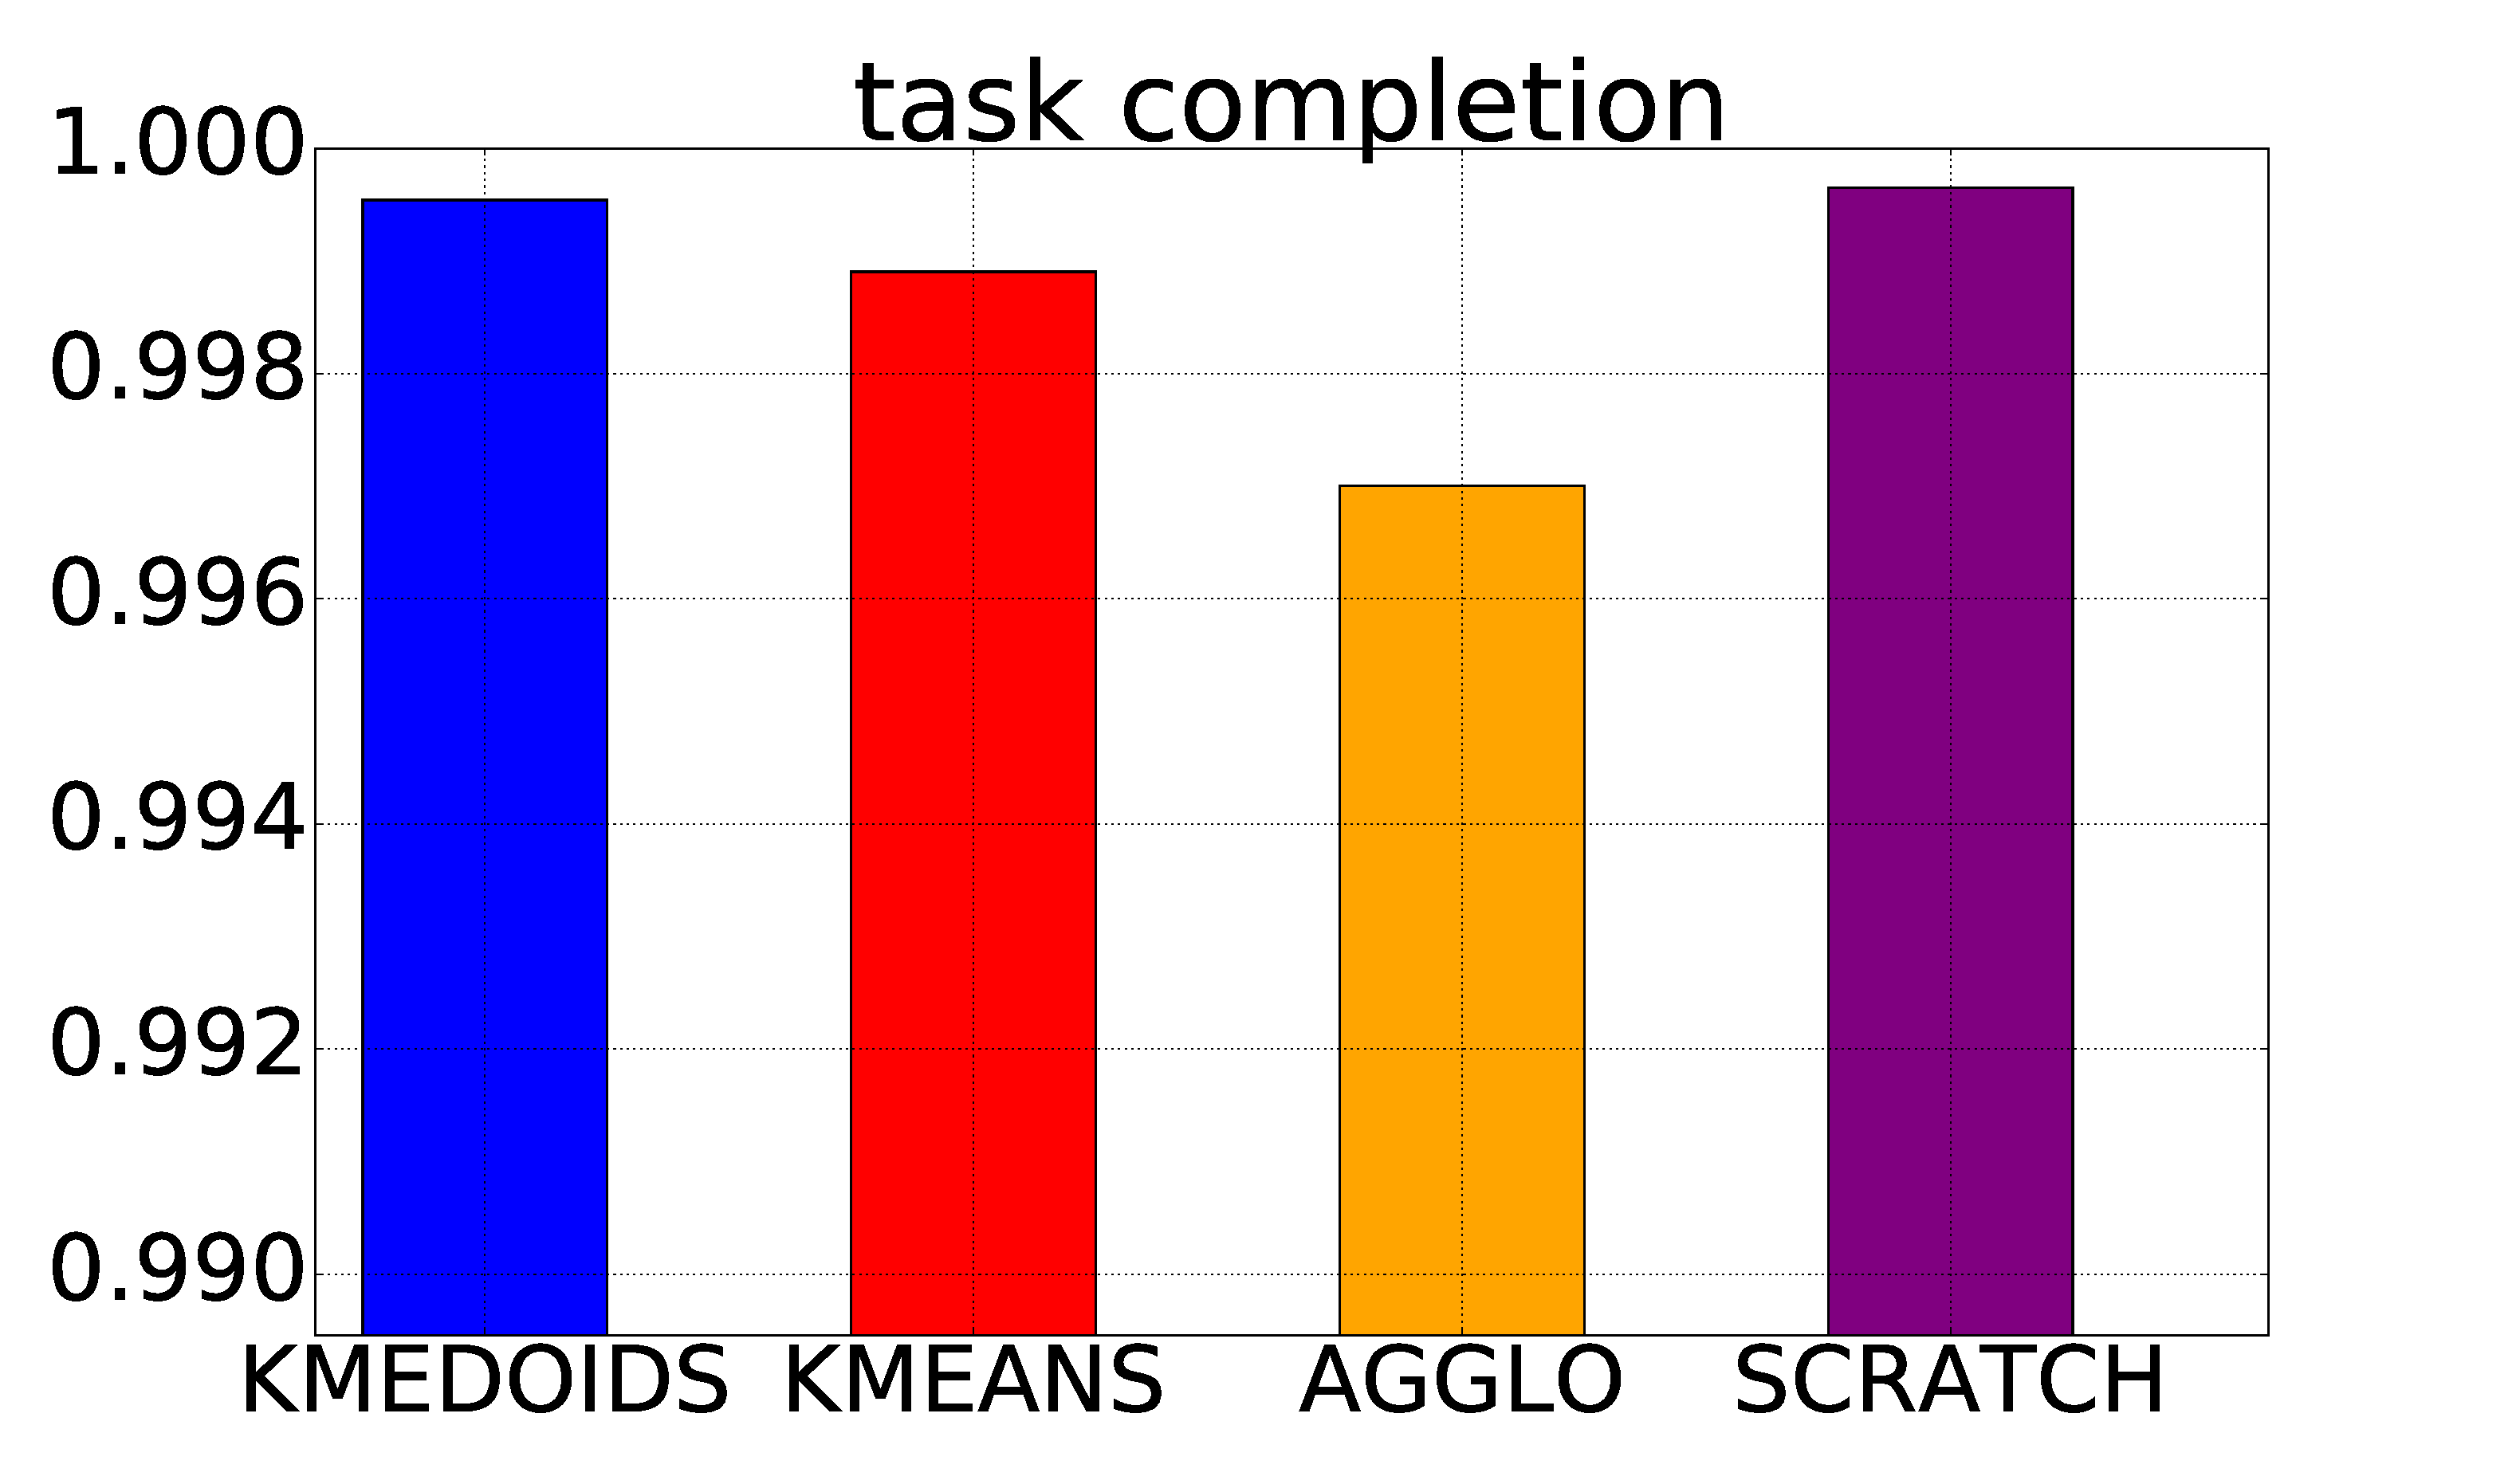
\includegraphics[width=0.33\textwidth]{img/handcraftedTC.pdf}
                }
            \end{center}
            \caption{Adaptation}
        \end{figure}
    \end{frame}

    \begin{frame}
        \begin{itemize}
            \item \cplus La solution fonctionne,
            \item \cmean mais beaucoup d'ingénierie:
            \begin{itemize}
                \item \cplus chaque composant peut être testé et validé,
                \item \cmoins chaque composant générère des approximations et erreurs,
                \item \cmoins effort de développement important,
                \item \cmoins meta paramètres.
            \end{itemize}
        \end{itemize}
        \pause
        Et si on pouvait
        \begin{itemize}
            \item \cplus avoir une solution \textit{scalable} naturellement,
            \item \cplus embarquée directement dans un algorithme \textit{low-level}.
        \end{itemize}
        \begin{exampleblock}{Solution}
            Transfer Deep Q-Learning (TDQN)
        \end{exampleblock}
        $\rightarrow$ Pas abordé dans cette présentation.
    \end{frame}



    \section{Apprentissage par transfert sécurisé}


    \begin{frame}

        \begin{alertblock}{Limitation}
            Nouvel utilisateur $\rightarrow$ risque d'abandon élevé.
        \end{alertblock}


        \begin{exampleblock}{Solution}
            \begin{itemize}
                \item Apprentissage de la politique de dialogue,
                \item sans "brusquer" l'utilisateur,
                \item en utilisant une politique sécurisée.
                \begin{itemize}
                    \item Notion de budget $\beta$: maîtrise du risque de raccrochage.
                \end{itemize}
            \end{itemize}
        \end{exampleblock}

    \end{frame}



    \subsection{Maîtrise du risque en RL}

    \begin{frame}

        \begin{block}{Raccrochage}
            $C:S\times A \rightarrow \{0,1\}$.
        \end{block}

        \begin{block}{Relaxation lagrangienne}
            $R \leftarrow R - \lambda C$.
        \end{block}


        \begin{alertblock}{Limitation}
            Quel $\lambda$ pour quel budget $\beta$?
        \end{alertblock}

        \begin{exampleblock}{Solution: calibration de $\lambda$}% oral: limitation des politiques lagragiennes
            On cherche notre politique sécurisée sur le front de pareto
        \end{exampleblock}


    \end{frame}

    \foreach \n in {0,1}{
    \begin{frame}{}
        \begin{figure}
            \begin{center}
                \includegraphics[width=1\textwidth]{drawio/out/pareto\n.pdf}
            \end{center}
        \end{figure}
    \end{frame}
    }

    \begin{frame}
        \begin{alertblock}{Limitations}
            \begin{itemize}
                \item \cmoins Processus lourd et approximatif % où commencer, quel steps ?
                \item \cmoins Il se peut qu'il n'existe pas de $\lambda$ pour $\beta$.
                \item \cmoins Formulation linéaire + déterminisme $\rightarrow$ comportements extrêmes.
                % pas de formulation linéaire de la reward pour un budget donné
            \end{itemize}
        \end{alertblock}
        \begin{exampleblock}{Solution}
            Budgeted Reinforcement Learning.
            % Ce qui nous amène à la prochaine contribution: BRL
        \end{exampleblock}
    \end{frame}


    \begin{frame}{Cadre}
        \begin{block}{Processus de Decision Markovien (MDP)}
            \begin{itemize}
                \item $(\cS, \cA, P, R, \gamma)$
                \item $G_r^\pi = \sum_{t=0}^\infty \gamma^t R(s_t, a_t)$ le retour des récompenses.
                \item Trouver $\pi^*$ t.q $\forall s\in\cS$:
                \begin{equation}
                    \label{eq:mdp}
                    \begin{array}{lcr}
                        \displaystyle \pi^* \in \argmax_{\pi\in\cM(\cA)^\cS} \expectedvalue[G_r^\pi | s_0=s]
                    \end{array}
                \end{equation}

            \end{itemize}
        \end{block}


        \begin{block}{}
            \begin{itemize}
                \item \cplus \textit{Tractable}
                \item \cmoins Comportements extrêmes
                \item \cmoins Calibration nécessaire (quel $\lambda$ pour $\beta$?)
                % A l ORAL si formulation sous contrainte
            \end{itemize}
        \end{block}

    \end{frame}

    \begin{frame}{Cadre}

        \begin{block}{Processus de Decision Markovien \textcolor{blue}{sous Contrainte} (CMDP)}
            \begin{itemize}
                \item $(\cS, \cA, P, R,\textcolor{blue}{C}, \gamma,\textcolor{blue}{\beta})$
                \item $G_r^\pi = \sum_{t=0}^\infty \gamma^t R(s_t, a_t)$ le retour des récompenses.
                \item \textcolor{blue}{ $G_c^\pi = \sum_{t=0}^\infty \gamma^t C(s_t, a_t)$ le retour des coûts.}
                \item Trouver $\pi^*$ t.q $\forall s\in\cS$:
                \begin{equation}
                    \label{eq:cmdp}
                    \begin{array}{lcr}
                        \displaystyle \pi^* \in \argmax_{\pi\in\cM(\cA)^\cS} \expectedvalue[G_r^\pi | s_0=s] \\
                        \text{ s.t. }  \textcolor{blue}{\expectedvalue[G_c^\pi | s_0=s] \leq \beta}
                    \end{array}
                \end{equation}
            \end{itemize}
        \end{block}

        \begin{block}{}
            \begin{itemize}
                \item \cplus \textit{Tractable}
                \item \cmean DOF supplémentaire (si mixture de politiques) % A L ORAL On peut définir un budget de safety , formuation plus naturelle
                \item \cmoins budget fixé
                % A L ORAL si le budget change on the fly, ou qu'il n'est pas adapté, on doit reapprendre une politique,  Or Le front de pareto est rarement linéaire, le choix du budget n'est pas évident


            \end{itemize}
        \end{block}

    \end{frame}

    \begin{frame}{Cadre}

        \begin{block}{Processus de Decision Markovien \textcolor{blue}{Budgeté} (BMDP)}
            \begin{itemize}
                \item $(\cS, \cA, P, R,{C}, \gamma,\textcolor{blue}{\cB})$
                \item $G_r^\pi = \sum_{t=0}^\infty \gamma^t R(s_t, a_t)$ le retour des récompenses.
                \item  $G_c^\pi = \sum_{t=0}^\infty \gamma^t C(s_t, a_t)$ le retour des coûts.
                \item Trouver $\pi^*$ t.q $\forall (s,\textcolor{blue}{\beta})\in\cS\times\textcolor{blue}{\cB}$:
                \begin{equation}
                    \label{eq:bmdp}
                    \begin{array}{lcr}
                        \displaystyle \pi^* \in \argmax_{\pi\in\cM(\cA\times\textcolor{blue}{\cB})^{\cS\times\textcolor{blue}{\cB}}} \expectedvalue[G_r^\pi | s_0=s,\textcolor{blue}{\beta_0=\beta}] \\
                        \text{ s.t. }  \expectedvalue[G_c^\pi | s_0=s,\textcolor{blue}{\beta_0=\beta}] \leq \beta
                    \end{array}
                \end{equation}
            \end{itemize}
        \end{block}


        \begin{block}{}
            \begin{itemize}
                \item \cmoins \textit{Non Tractable}
                \item \cplus DOF supplémentaire
                \item \cplus budget non fixé

                % A L ORAL On peut définir un budget de safety et d'afranchir des lambda.}
            \end{itemize}
        \end{block}

    \end{frame}


    \begin{frame}{Cadre augmenté}

        \textbf{Politique budgeté} $\pi\in\Pi$
        \begin{itemize}
            \item $ \pi:\underbrace{(s,\beta)}_{\os} \rightarrow \underbrace{(a,\beta')}_{\oa}$
        \end{itemize}

        \textbf{Domain}
        \begin{itemize}
            \item Etats $\ocS = \cS\times\cB$.
            \item Actions $\ocA = \cA\times\cB$.
            \item Dynamique $\ov{P}$
            %$\left((s',\beta') \condbar (s,\beta), (a, \beta_a)\right) \eqdef P(s'|s, a)\delta(\beta' - \beta_a)$.
        \end{itemize}
        \textbf{2D signals}
        \begin{itemize}
            \item Récompenses $\ov{R} = (R, C)$
            \item Retours $G^\pi = (G_r^\pi, G_c^\pi)$
            \item $V^\pi(\os) = (V_r^\pi, V_c^\pi) \eqdef \expectedvalue\left[ G^\pi \condbar \ov{s_0} = \os\right]$
            \item $Q^\pi(\os, \oa)= (Q_r^\pi, Q_c^\pi) \eqdef \expectedvalue\left[ G^\pi \condbar \ov{s_0} = \os, \ov{a_0} = \oa\right]$
        \end{itemize}

    \end{frame}

    \begin{frame}{Optimalité}
        \begin{definition}
            \begin{enumerate}
                \item[(i)] \pause\colorbox{red}{Respecter le budget $\beta$}:
                \begin{equation*}
                    \Pi_a(\os) \eqdef \{\pi\in\Pi: V_c^\pi(s, \beta) \mathcolorbox{red}{\leq \beta}\}
                \end{equation*}
                \item[(ii)] \pause\colorbox{green}{Maximiser les récompenses}:
                \begin{equation*}
                    V_r^*(\os) \eqdef \mathcolorbox{green}{\max}_{\pi\in\Pi_a(\os)}  V_r^\pi(\os) \qquad\quad \Pi_r(\os) \eqdef \mathcolorbox{green}{\argmax}_{\pi\in\Pi_a(\os)}  V_r^\pi(\os)
                \end{equation*}
                \item[(iii)] \pause\colorbox{yellow}{Minimiser les coûts}:
                \begin{equation*}
                    V_c^*(\os) \eqdef \mathcolorbox{yellow}{\min}_{\pi\in\Pi_r(\os)}  V_c^\pi(\os), \qquad\quad \Pi^*(\os) \eqdef \mathcolorbox{yellow}{\argmin}_{\pi\in\Pi_r(\os)}  V_c^\pi(\os)
                \end{equation*}
            \end{enumerate}

            \pause On défini $Q^*$ de la même façon.
        \end{definition}
    \end{frame}

    \begin{frame}{Equation d'optimalité de Bellman}
        \begin{block}{Equation d'optimalité de Bellman}
            $Q^*$ vérifie:
            \begin{align*}
                Q^{*}(\os, \oa) &= \cT Q^{*}(\os, \oa)\\
                &\eqdef \ov{R}(\os, \oa) + \gamma \sum_{\os'\in\ocS} \ov{P}(\ov{s'} | \os, \oa)\sum_{\ov{a'}\in \ocA} \pi_\text{greedy}(\ov{a'}|\ov{s'}; Q^*) Q^{*}(\ov{s'}, \ov{a'}),
            \end{align*}
            avec:\pause
            \begin{align*}
                \pi_\text{greedy}(\cdot|\os; Q) \in &\mathcolorbox{yellow}{\argmin}_{\rho\in\Pi_r^Q} \sum_{\oa}\rho(\oa) Q_c(\os, \oa), \\
                \text{where }\quad \Pi_r^Q \eqdef &\mathcolorbox{green}{\argmax}_{\rho\in\cM(\ocA)} \sum_{\oa}\rho(\oa) Q_r(\os, \oa) \\
                & \text{ s.t. }   \sum_{\oa}\rho(\oa) Q_c(\os, \oa) \mathcolorbox{red}{\leq \beta}
            \end{align*}
        \end{block}
        % ORAL: comment résoudre ce problème ?
    \end{frame}


    \foreach \n in {0,1,2,3,4}{
    \begin{frame}{Résoudre le problème non linéaire}
        \begin{figure}
            \centering
            %%\vspace{-1.5em}
            \includegraphics[scale=1.0,page=1]{img/b\n}
        \end{figure}
    \end{frame}
    }

    \begin{frame}{Comportement asymptotique}


        \begin{alertblock}{ \cmoins $\cT$ n'est pas une contraction:}
            $\forall\epsilon>0, \exists Q^1,Q^2\in(\Real^2)^{\ocS\ocA}:\|\cT Q^1-\cT Q^2\|_\infty \geq \frac{1}{\epsilon}\|Q^1-Q^2\|_\infty$
        \end{alertblock}

        \begin{exampleblock}{\cplus sauf quand les $Q$-fonctions sont lisses:}
            $\cT$ est une contraction pour le sous-ensemble $\cL_\gamma$ des $Q$-fonctions tel que "$Q_r$ est $L$-Lipschitz par rapport $Q_c$", avec $L<\frac{1}{\gamma}-1$

        \end{exampleblock}
    \end{frame}

    \begin{frame}

        \begin{block}{Budgeted Value-Iteration}
            \begin{itemize}
                \item $Q \leftarrow \mathbf{0}$
                \item $Q(\os,\oa) \leftarrow \bo Q(\os,\oa)\ \forall (\os,\oa)$ jusqu'à convergence % peut ne pas arriver
                \item Return $\pi(\os) = \pi_\text{greedy}(\cdot|\os; Q)$
            \end{itemize}
        \end{block}
        \pause
        \begin{alertblock}{}
            \begin{itemize}
                \item Comment calculer $\bo Q$ si $\transition$, $\reward$ et $\constraint$ sont inconnues?
                \begin{itemize}
                    \item Estimateur avec $\mathcal{D}=\{(\os_i,\oa_i,\ov{r}_i',\os_i')\}_{i\in[0,N]}$
                \end{itemize}
                \item Comment calculer $Q\ \forall (\os,\oa) \in \ocS\times\ocA$ si $\ocS$ est très grand voir continu ?
                \begin{itemize}
                    \item Approximation de fonction
                \end{itemize}
            \end{itemize}

        \end{alertblock}
        \pause
        \begin{block}{Budgeted Fitted-Q}
            \begin{itemize}
                \item $Q \leftarrow \mathbf{0}$
                \item $Q \leftarrow \Gamma(\{\os_{\indextransition},\oa_{\indextransition}\}_{{\indextransition}\in \T},\{\ov{r}'_{\indextransition} + \gamma \sum_{\ov{a}'\in \cA} \pi_\text{greedy}(\ov{a}'|\ov{s}'_{\indextransition}; Q) Q(\ov{s}'_{\indextransition}, \ov{a}')_{{\indextransition} \in \T}\})$
                \item Return $\pi(\os) = \pi_\text{greedy}(\cdot|\os; Q)$
            \end{itemize}
        \end{block}
    \end{frame}

    \begin{frame}{Exploration Risk-sensitive}

        Comment construire $\cD$?

        \begin{exampleblock}{Solution}
            Exploration avec Risk-sensitive $\epsilon$-greedy
        \end{exampleblock}
        $\rightarrow$ Pas abordée dans cette présentation
    \end{frame}

    \begin{frame}{Expériences}

        \begin{block}{Environnement}

            Remplissage d'un formulaire

            \begin{itemize}
                \item \texttt{ask-next}%: ask next slot (with ASR errors).
                \item \texttt{repeat-oral} (sécurisé + erreurs ASR)%: repeat current slot (with ASR errors).
                \item \texttt{repeat-numpad} (risqué)%: repeat current slot using numeric pad (without ASR errors).
                \item \texttt{summarize-inform}
                %: summarise slots values and return the form result. If values are correct, the dialogue ends successfully, if not, the slot values are reset and the dialogue continues from the first slot.
            \end{itemize}


        \end{block}
    \end{frame}

    \begin{frame}{Expériences}
        \begin{center}
            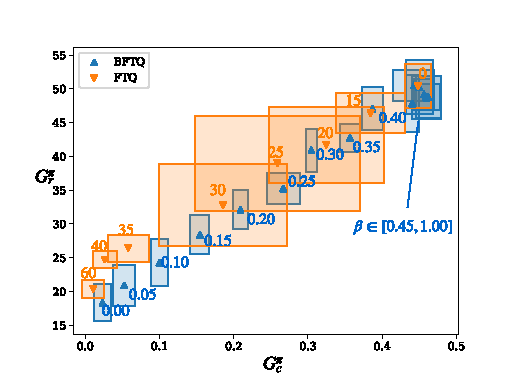
\includegraphics[width=0.75\textwidth]{img/slot-filling.pdf}
        \end{center}
    \end{frame}



    \begin{frame}{Pour aller plus loin}

        \begin{itemize}
            \item Les récompenses en dialogue sont très \textit{sparse}.
            \item Et si on utilisait une politique sécurisée pour découvrir plus de récompenses?
        \end{itemize}

        \begin{exampleblock}{Solution}
            Transfert avec $\epsilon$- safe
        \end{exampleblock}
        $\rightarrow$ Pas abordée dans cette présentation
    \end{frame}
    %    \subsection{$\epsilon$-safe}
    %    \begin{frame}{$\epsilon$- safe}
    %        Pas abordé dans cette présentation.
    %    \end{frame}

    \section{Conclusion et perspectives}
    \begin{frame}{Conclusion}
        \begin{itemize}
            \item Prise de décision dans un SDS = le gestionnaire de dialogue
            \item Formulation avec du RL
            \item Comment s'adapater rapidement à un nouvel utilisateur ?
            \begin{itemize}
                \item Apprentissage par transfert
            \end{itemize}
            \item Deux directions:
            \begin{itemize}
                \item Mise à l'échelle de solutions existantes
                \begin{itemize}
                    \item PD-distance: Clustering de politiques
                    \item TDQN: Solution de transfert en continu avec DQN (pas abordé ici)
                \end{itemize}
                \item Approche sécurisée:
                \begin{itemize}
                    \item formulation lagragienne insuffisante $\rightarrow$ Budgeted-RL
                    \item $\epsilon$-safe (pas abordé ici)
                \end{itemize}
            \end{itemize}
        \end{itemize}
    \end{frame}

    \begin{frame}{Perspectives}
        \begin{itemize}
            \item Co-adaptation
            \item Multi-agents
%            \item Nouvelles notions de sureté % induction en erreur,
        \end{itemize}

    \end{frame}

    %    \begin{frame}
    %        \printbibliography[heading=bibempty]
    %
    %    \end{frame}

\end{document}

